%--------------------------------------------------------------------%
%
% Berkas utama templat LaTeX.
%
% author Petra Barus, Peb Ruswono Aryan, Faris Rizki Ekananda
%
%--------------------------------------------------------------------%
%
% Berkas ini berisi struktur utama dokumen LaTeX yang akan dibuat.
%
%--------------------------------------------------------------------%

\documentclass[bahasa, 12pt, a4paper, onecolumn, oneside, final]{report}

%-------------------------------------------------------------------%
%
% Konfigurasi dokumen LaTeX untuk laporan tesis IF ITB
%
% @author Petra Novandi
%
%-------------------------------------------------------------------%
%
% Berkas asli berasal dari Steven Lolong
%
%-------------------------------------------------------------------%

% Ukuran kertas
\special{papersize=210mm,297mm}

% Setting margin
\usepackage[top=2cm,bottom=2cm,left=4cm,right=3cm]{geometry}
% Underline
\usepackage[normalem]{ulem}

\usepackage{mathptmx}

% Judul bahasa Indonesia
\usepackage[bahasa]{babel}

% Format citation
\usepackage[utf8]{inputenc}
\usepackage[style=apa,backend=biber]{biblatex}

\usepackage{graphicx}
\usepackage{titling}
\usepackage{blindtext}
\usepackage{sectsty}
\usepackage{chngcntr}
\usepackage{etoolbox}
\usepackage{array}
\usepackage[hidelinks]{hyperref}       % Package untuk link di daftar isi. Ubah jadi \usepackage[hidelinks]{hyperref} apabila ingin menghilangkan kotak merah disekitar link
\usepackage{titlesec}       % Package Format judul
\usepackage{titletoc}       % Package Format judul di toc
\usepackage{tocbibind}      % Package untuk masukkan toc, lot, lof ke Daftar Isi
\usepackage{scrwfile}       % Package untuk membuat Daftar Lampiran dari toc
\usepackage{parskip}
\usepackage{afterpage}
\usepackage{relsize}
\usepackage{longtable}
\usepackage{colortbl}
\usepackage[dvipsnames]{xcolor}
\usepackage{setspace}
\usepackage{booktabs}
\usepackage{pgfgantt} 
\usepackage{geometry}	% for page margin settings
\usepackage{pdflscape}	% for landscape orientation
\usepackage{enumitem}	% itemize
\usepackage{multirow}	% joining row
\usepackage{xspace}	% spacing for macros
\usepackage{caption}	% table and figure caption spacing
% Daftar Istilah
\usepackage{tabularx}
% Codeblocks
\usepackage{listings}
% Dir tree
\usepackage{tikz}
\usepackage{forest}
% Equation
\usepackage{amsmath}

\graphicspath{{resources/}}   % letak direktori penyimpanan gambar

% Setting daftar lampiran
\newcommand*{\lopname}{DAFTAR LAMPIRAN}
\TOCclone[\lopname]{toc}{atoc}
\addtocontents{atoc}{\protect\value{tocdepth}=-1}
\newcommand\listofappendices{
  \cleardoublepage
  \phantomsection
  \listofatoc
  \addcontentsline{toc}{chapter}{\lopname}
}

\newcommand*\savedtocdepth{}
\AtBeginDocument{%
  \edef\savedtocdepth{\the\value{tocdepth}}%
}

\let\originalappendix\appendix
\renewcommand\appendix{%
  \originalappendix
  \cleardoublepage
  \addtocontents{toc}{\protect\value{tocdepth}=-1}%
  \addtocontents{atoc}{\protect\value{tocdepth}=\savedtocdepth}%

  \titlecontents{chapter}
    [0pt]
    {\bfseries}
    {Lampiran \thecontentslabel.\quad}
    {}
    {\hfill\contentspage}

  \titleformat{\chapter}[block]
    {\bfseries}
    {\chaptertitlename\ \thechapter.\quad}{0pt}
    {\bfseries}
}

% Hilangkan titik pada toc
\makeatletter
\renewcommand{\@dotsep}{1} 
\makeatother

% Setel title pada chapter-chapter di toc, lof, lot
\titlecontents{chapter}
  [0pt]
  {\bfseries}
  {\MakeUppercase{Bab} \thecontentslabel\quad\uppercase}
  {}
  {\mdseries\titlerule*[0.35em]{.}\bfseries\contentspage}
\titlecontents{figure}
  [0pt]
  {}
  {Gambar \thecontentslabel.\quad}
  {}
  {\mdseries\titlerule*[0.35em]{.}\bfseries\contentspage}
\titlecontents{table}
  [0pt]
  {}
  {Tabel \thecontentslabel.\quad}
  {}
  {\mdseries\titlerule*[0.35em]{.}\bfseries\contentspage}

% Masukin Daftar Pustaka ke toc
\let\originalprintbibliography\printbibliography
\renewcommand\printbibliography{%
  \phantomsection
  \cleardoublepage
  \originalprintbibliography
  \addcontentsline{toc}{chapter}{\bibname}
}

% Line satu setengah spasi
\renewcommand{\baselinestretch}{1.5}

% Setting judul
\chapterfont{\centering \large}
\titleformat{\chapter}[display]
  {\Large\centering\bfseries}
  {\chaptertitlename\ \thechapter}{0pt}
    {\Large\bfseries\uppercase}

% Setting nomor pada subbsubsubbab
\setcounter{secnumdepth}{3}

\makeatletter

\makeatother

% Counter untuk figure dan table.
\counterwithin{figure}{chapter}
\counterwithin{table}{chapter}

% Define blank page
\newcommand*{\blankpage}{\afterpage{\null\newpage}}

% Translate autoref into Indonesian
\renewcommand*{\equationautorefname}{Persamaan}%
\renewcommand*{\footnoteautorefname}{catatan kaki}%
\renewcommand*{\itemautorefname}{item}%
\renewcommand*{\figureautorefname}{Gambar}%
\renewcommand*{\tableautorefname}{Tabel}%
\renewcommand*{\partautorefname}{Bagian}%
\renewcommand*{\appendixautorefname}{Lampiran}%
\renewcommand*{\chapterautorefname}{Bab}%
\renewcommand*{\sectionautorefname}{Subbab}%
\renewcommand*{\subsectionautorefname}{Subsubbab}%
\renewcommand*{\subsubsectionautorefname}{Subsubsubbab}%
\renewcommand*{\paragraphautorefname}{paragraf}%
\renewcommand*{\subparagraphautorefname}{subparagraf}%
\renewcommand*{\FancyVerbLineautorefname}{garis}%
\renewcommand*{\theoremautorefname}{Teorema}%
\renewcommand*{\pageautorefname}{halaman}%

% Setting codeblocks
\definecolor{mygreen}{rgb}{0,0.6,0}
\definecolor{mygray}{rgb}{0.5,0.5,0.5}
\definecolor{mymauve}{rgb}{0.58,0,0.82}

\lstset{ 
  backgroundcolor=\color{white},   % choose the background color; you must add \usepackage{color} or \usepackage{xcolor}; should come as last argument
  basicstyle=\ttfamily\footnotesize,        % the size of the fonts that are used for the code
  breakatwhitespace=false,         % sets if automatic breaks should only happen at whitespace
  breaklines=true,                 % sets automatic line breaking
  captionpos=b,                    % sets the caption-position to bottom
  commentstyle=\color{mygreen},    % comment style
  escapeinside={\%*}{*)},          % if you want to add LaTeX within your code
  extendedchars=true,              % lets you use non-ASCII characters; for 8-bits encodings only, does not work with UTF-8
  frame=single,	                   % adds a frame around the code
  keepspaces=true,                 % keeps spaces in text, useful for keeping indentation of code (possibly needs columns=flexible)
  keywordstyle=\color{blue},       % keyword style
  rulecolor=\color{black},         % if not set, the frame-color may be changed on line-breaks within not-black text (e.g. comments (green here))
  showspaces=false,                % show spaces everywhere adding particular underscores; it overrides 'showstringspaces'
  showstringspaces=false,          % underline spaces within strings only
  showtabs=false,                  % show tabs within strings adding particular underscores
  stringstyle=\color{mymauve},     % string literal style
  tabsize=2,	                   % sets default tabsize to 2 spaces
  title=\lstname                   % show the filename of files included with \lstinputlisting; also try caption instead of title
}

% Setting forest
\forestset{default preamble={tikz+={\tikzset{show background rectangle}}}}


\makeatletter

\makeatother

\addbibresource{references.bib}

\begin{document}

%Basic configuration
\title{Peningkatan Kinerja IndoBERT dengan Menggunakan Berbagai Metode \textit{Parameter-Efficient Transfer Learning}}
\date{} 
\author{
    Adiyansa Prasetya Wicaksana \\
    NIM: 13520044
}
\newcommand\tanggalpengesahan{DD MMMM 2024}

\pagenumbering{roman}
\setcounter{page}{1}

\clearpage
\pagestyle{empty}

\begin{center}
    \smallskip
    
    \Large \bfseries \MakeUppercase{\thetitle}
    \vfill
    
    \Large Laporan Tugas Akhir
    \vfill
    
    \large Disusun sebagai syarat kelulusan tingkat sarjana
    \vfill
    
    \large Oleh
    
    \Large \theauthor
    
    \vfill
    \begin{figure}[h]
        \centering
        \includegraphics[width=0.15\textwidth]{cover-ganesha.jpg}
    \end{figure}
    \vfill
    
    \large
    \uppercase{
        Program Studi Teknik Informatika \\
        Sekolah Teknik Elektro \& Informatika \\
        Institut Teknologi Bandung
    }
    
    Desember 2023
    
\end{center}

\clearpage

\clearpage
\pagestyle{empty}

\begin{center}
    \smallskip
    
    \Large \bfseries \MakeUppercase{\thetitle}
    \vfill
    
    \Large Laporan Tugas Akhir 1
    \vfill
    
    \large Oleh
    
    \Large \theauthor
    
    \large Program Studi Teknik Informatika \\
    
    \normalsize \normalfont
    Sekolah Teknik Elektro dan Informatika \\
    Institut Teknologi Bandung \\
    
    \vfill
    \normalsize \normalfont
    Bandung, 15 Desember 2023 \\
    Mengetahui,
    
    \vspace{0.5cm}
    Pembimbing,
    
    \vfill
    \underline{Dr. Fariska Zakhralativa Ruskanda, S.T., M.T.} \\
    NIP. 119 110 075
    
\end{center}
\clearpage

\chapter*{Lembar Pernyataan}

Dengan ini saya menyatakan bahwa:

\begin{enumerate}

    \item Pengerjaan dan penulisan Laporan Tugas Akhir ini dilakukan tanpa menggunakan bantuan yang tidak dibenarkan.
    \item Segala bentuk kutipan dan acuan terhadap tulisan orang lain yang digunakan di dalam penyusunan laporan tugas akhir ini telah dituliskan dengan baik dan benar.
    \item Laporan Tugas Akhir ini belum pernah diajukan pada program pendidikan di perguruan tinggi mana pun.

\end{enumerate}

Jika terbukti melanggar hal-hal di atas, saya bersedia dikenakan sanksi sesuai dengan Peraturan Akademik dan Kemahasiswaan Institut Teknologi Bandung bagian Penegakan Norma Akademik dan Kemahasiswaan khususnya Pasal 2.1 dan Pasal 2.2.
\vspace{15mm}

Bandung, \tanggalpengesahan

\vspace{1.5cm}
Adiyansa Prasetya Wicaksana \\
NIM 13520044


\pagestyle{plain}

\clearpage
\chapter*{ABSTRAK}
\addcontentsline{toc}{chapter}{Abstrak}

\begin{center}
    \center
    \begin{singlespace}
        \large\bfseries\MakeUppercase{\thetitle}
    
        \normalfont\normalsize
        Oleh
    
        \bfseries \theauthor
    \end{singlespace}
\end{center} 

\begin{singlespace}
    Metode \textit{fine-tuning}  selalu digunakan sebagai metode pelalihan untuk melakukan evaluasi pada berbagai evaluasi NLU. Kakas evaluasi IndoLEM yang merupakan pionir dari evaluasi NLU berbahasa Indonesia menggunakan \textit{fine-tuning} sebagai metode pelatihannya. \textit{Fine-tuning} melatih model dengan mengubah seluruh paramter model. Hal ini bisa menjadi tantangan dari segi memori dan juga waktu pelatihannya. Terdapat metode \PEFT yang dapat melatih model dengan kinerja yang sebanding dengan metode \textit{fine-tuning} . Dalam tugas akhir ini, berbagai metode \PEFT, yaitu \methodPEFT dimaanfaatkan dalam kakas evaluasi IndoLEM tersebut.
\end{singlespace}

\clearpage

% \clearpage
\chapter*{ABSTRACT}
\addcontentsline{toc}{chapter}{ABSTRACT}

\begin{center}
    \center
    \begin{singlespace}
        \large\bfseries\MakeUppercase{\titleen}
    
        \normalfont\normalsize
        By:
    
        \bfseries \theauthor
    \end{singlespace}
\end{center} 

\begin{singlespace}
    The fine-tuning method is employed as a training approach for evaluating various NLU tasks. IndoLEM, which is a pioneer in the evaluation of Indonesian-language NLU, uses fine-tuning as its training method. Fine-tuning involves training the model by modifying all of its parameters, which can be challenging in terms of memory and training time. There exists a method called PEFT that can train models with performance comparable to fine-tuning. In this thesis, various PEFT methods, namely \methodPEFT, are utilized in the evaluation tasks of IndoLEM. The aim of this thesis is to leverage PEFT methods in IndoLEM, including the incorporating of PEFT methods, performance comparisons for each PEFT method, and analysis of parameter usage and training time.
    This thesis successfully leverages PEFT methods on IndoLEM. Through refactoring of IndoLEM, PEFT methods were successfully incorporated. Subsequently, experiments were conducted by training models using both fine-tuning and PEFT methods. Testing was carried out on three evaluation tasks, namely \nlptask. The experimental results indicate that PEFT only uses approximately 0.2\% to 15\% of the model's training parameters, with faster training times. The performance achieved for the NER and sentiment analysis tasks ranged from -0.8\% to -6.2\%. This indicates a trade-off between the use of training parameters and the resulting performance. However, the Prefix-Tuning and UniPELT methods failed to provide consistent results on the summarization task.

    \textit{\textbf{Keywords: Fine-tuning, Parameter-efficient, IndoLEM, NER, Sentiment Analysis, Summarization}}
\end{singlespace}

\clearpage

\chapter*{KATA PENGANTAR}
\addcontentsline{toc}{chapter}{KATA PENGANTAR}

Puji dan syukur penulis panjatkan kepada Tuhan Yang Maha Esa atas berkat dan rahmatnya, laporan tugas akhir yang berjudul \thetitle{} dapat diselesaikan dalam rangka memenuhi syarat kelulusan tingkat sarjana. Perlu diakui pengerjaan tugas akhir ini didukung oleh banyak pihak. Khususnya, penulis ingin mengucapkan terima kasih kepada:

\begin{enumerate}
    \item{
            Ibu Dr. Fariska Zakhralativa Ruskanda, S.T., M.T. selaku dosen pembimbing tugas akhir atas segala bentuk bimbingan dan dukungan yang sangat membantu dalam pengerjaan tugas akhir ini.
        }
    \item{
            Dicky Prima Satya, S.T, M.T., Bapak Adi Mulyanto, S.T, M.T., Robithoh Annur, S.T., M.Eng., Ph.D., dan Tricya Esterina Widagdo, ST., M.Sc selaku dosen koordinator tim tugas akhir atas segala bentuk materi dan usahanya untuk mempermudah mahasiswa dalam pengerjaan tugas akhir. 
        }
    \item{
            Seluruh dosen program studi Teknik Informatika ITB atas segala bentuk ilmu yang telah diajarkan kepada mahasiswa. Semoga seluruh ilmu yang diajarkan bisa terus bermanfaat.
        }
    \item{
            Seluruh \textit{staff} fakultas STEI atas segala jasanya dalam memudahkan mahasiswa pada proses perkuliahan.
        }
    \item{
            Bapak Ade Hermawan dan Ibu Annik Oktaelly selaku orang tua atas segala doa dan bantuan yang bisa diberikan dalam pengerjaan tugas akhir ini. Anggun dan Dean, selaku saudara dari penulis atas segala dukungannya. Semoga semua hal baik selalu menyertai mereka.
        }
    \item{
            Sahabat terbaik, Trista, yang selalu menemani dan memberikan dukungan yang terbaik setiap saatnya.
        }
    \item{
            Sahabat terdekat dari SMA, Haffif, Samuel, Kiagus, Patria, Aji, Adit, Yoga, Mak, Rafy, Revan, Ocit, Reyhan, Vigar, Aysar, Hanip dan sahabat-sahabat lainnya dari SMA atas seluruh memori dan pelajaran hidup yang diberikan.
        }
    \item{
            Sahabat terdekat dari perkuliahan, Gagas, Dhika, Gare, Kinan, Marcho, Aira, Dipa, Januar, Ubai, Fikri, Fikron, Kibar, Eja, Azka, Azka, Epi, Ken, Arik, Fikri, Kevin, Ocep, Shadiq, Jova, Saul, Chus, Hanip, Kosar, Adila, dan teman-teman lainnya dari perkuliahan atas seluruh kenangan, obrolan, dan pelajaran hidup yang diberikan.
        }
    \item{
            Seluruh pihak lainnya yang tidak bisa disebutkan yang secara tidak langsung ataupun langsung membantu pengerjaan tugas akhir ini.
        }
\end{enumerate}

Akhir kata, penulis mengucapkan terima kasih kepada semua pihak yang telah terlibat dalam pengerjaan tugas akhir ini. Penulis juga ingin menyampaikan mohon maaf apabila terdapat kesalahan maupun kekurangan dalam laporan tugas akhir ini. Penulis berharap semoga tugas akhir ini dapat bermanfaat bagi pembaca dan riset-riset ke depannya.

\begin{flushright}
    \vspace{0.5cm}
    Bandung, \tanggalpengesahan


    \vspace{1.5cm}

    Adiyansa Prasetya Wicaksana
\end{flushright}


\titlespacing*{\chapter}{0pt}{0pt}{4pt}

% Setting judul toc, lot, lof, bib
\renewcommand{\contentsname}{DAFTAR ISI}
\renewcommand{\listfigurename}{DAFTAR GAMBAR}
\renewcommand{\listtablename}{DAFTAR TABEL}
\renewcommand{\bibname}{DAFTAR PUSTAKA}

\tableofcontents
\listofappendices
\listoffigures
\listoftables

\newpage

\titleformat*{\section}{\bfseries\large}
\pagenumbering{arabic}

%----------------------------------------------------------------%
% Konfigurasi Bab
%----------------------------------------------------------------%
\setcounter{page}{1}
\renewcommand{\chaptername}{BAB}
\renewcommand{\thechapter}{\Roman{chapter}}
%----------------------------------------------------------------%

%----------------------------------------------------------------%
% Dafter Bab
% Untuk menambahkan daftar bab, buat berkas bab misalnya `chapter-6` di direktori `chapters`, dan masukkan ke sini.
%----------------------------------------------------------------%
\chapter{Pendahuluan}

Bab ini berisi terkait gambaran umum dan permasalahan yang akan diselesaikan dalam tugas akhir ini. Bab ini akan dimulai dari penjelasan latar belakang dari masalah yang diselesaikan, rumusan masalah, tujuan, batasan masalah, metodologi yang digunakan, dan berakhir pada sistematika penulisan tugas akhir ini.

\section{Latar Belakang}
\label{sec:latar-belakang}

Pengolahan bahasa alami (\textit{Natural Language Processing}, NLP) telah menjadi salah satu bidang yang mengalami perkembangan pesat. Kemampuan untuk memahami, menginterpretasi, dan merespons bahasa manusia secara bermakna telah membuka berbagai aplikasi baru yang inovatif. Pengaplikasian bahasa alami mencakup berbagai aspek, mulai dari pemahaman teks (seperti \textit{text classification} dan \textit{sentiment analysis}), hingga generasi bahasa (seperti \textit{machine translation}).

Kemampuan bahasa dari manusia bersifat umum dan fleksible. Sebaliknya, evaluasi kemampuan pemahaman bahasa (\textit{natural language understanding}, NLU) dari NLP perlu menjalankan berbagai tugas linguistik pada berbagai domain \parencite{glue}. Untuk mengatasi masalah ini, terdapat banyak kakas dan korpora yang telah diajukan. Salah satunya adalah GLUE (\textit{General Language Understanding Evaluation}) \parencite{glue} dan SuperGLUE \parencite{superglue} untuk mengevaluasi NLU dalam bahasa Inggirs. GLUE meliputi 9 tugas evaluasi, sedangkan SuperGLUE merupakan jenis evaluasi yang lebih sulit dari GLUE yang memiliki delapan tugas evaluasi \parencite{indolem}.

Untuk evaluasi pemahaman NLP dalam bahasa Indonesia, terdapat beberapa kakas yang telah diajukan, salah satunya dalah IndoLEM \parencite{indolem}, IndoNLU \parencite{indonlu}, dan IndoNLG \parencite{indonlg}. IndoLEM merupakan kakas yang muncul dari ketiadaan kakas evaluasi NLU untuk bahasa Indonesia. IndoLEM terdiri dari 7 tugas, salah satunya adalah \textit{named entity recognition} (NER), \textit{sentiment analysis}, dan \textit{summarization} \parencite{indolem}. IndoNLU menyediakan 12 evaluasi NLU, sedangkan IndoNLG fokus terhadap evaluasi \textit{natural language generation} (NLG).

Dalam proses evaluasi NLU, model perlu dilatih pada \textit{dataset} yang tersedia pada kakas tersebut, lalu evaluasi bisa dilakukan dengan membandingkan hasil pelatihannya dengan \textit{benchmark} yang ada. Proses pelatihan ini menggunakan metode \textit{fine-tuning} \parencite{indolem}. Terdapat peluang untuk peningkatan lebih lanjut, terutama dalam hal efisiensi parameter yang digunakan dan waktu pelatihannya. Penggunaan \textit{fine-tuning} pada proses pelatihan, memerlukan sumber daya komputasi yang besar, yang tidak selalu tersedia atau praktis untuk semua pengguna. Salah satu pendekatan yang menjanjikan untuk mengatasi tantangan ini adalah penggunaan teknik \PEFT. PEFT memungkinkan model untuk menyesuaikan dengan tugas-tugas spesifik dengan mengubah jumlah parameter yang relatif kecil sehingga mempertahankan sebagian besar parameter model yang telah dilatih sebelumnya \parencite{adapter}. Teknik ini tidak hanya dapat mengurangi waktu dan biaya komputasi, tetapi juga memungkinkan penyesuaian model yang lebih cepat dan lebih fleksibel untuk aplikasi spesifik. 

Teknik \PEFT memiliki berbagai variasi, seperti LoRA (\textit{Low-Rank Adaptation}), \textit{Prefix-Tuning}, dan \textit{Bottleneck Adapter}. Penelitian yang dilakukan oleh \citeauthor{adapter} \parencite{adapter} dan \citeauthor{uvpl} \parencite{uvpl} menunjukkan bahwa dengan memperbarui kurang dari 4\% parameter, metode berbasis PEFT dapat mencapai kinerja yang sebanding dengan metode \textit{fine-tuning} penuh. Setiap teknik memiliki karakteristiknya sendiri, dan hingga saat ini, belum banyak penelitian yang secara komprehensif membandingkan kinerja antara teknik-teknik ini, terutama ketika diterapkan pada model IndoBERT. 

Tugas akhir ini akan difokuskan pada pemanfaatan berbagai teknik \PEFT pada kakas evaluasi IndoLEM dengan tujuan untuk mengimplementasikan berbagai metode PETL pada kakas evaluasi IndoLEM. Selain itu, tugas akhir ini akan membandingkan kinerja berbagai teknik \PEFT dengan metode \textit{fine-tuning} tradisional untuk mendapatkan metode mana yang paling efisien. Dengan demikian, tugas akhir ini ini diharapkan dapat memberikan kontribusi dalam pemanfaatan metode PEFTpada IndoLEM, sekaligus memberikan pemahaman yang lebih baik mengenai efisiensi berbagai teknik \PEFT dalam konteks bahasa Indonesia.

\section{Rumusan Masalah}

Dalam konteks pengembangan IndoBERT, penelitian ini akan menjawab beberapa pertanyaan utama, yaitu:

\begin{enumerate}
    \item Apakah berbagai metode \PEFT, yaitu \methodPEFT, dapat diimplementasikan pada kakas evaluasi IndoLEM?
    \item Apakah ada perbedaan signifikan dalam kinerja antara teknik-teknik \PEFT tersebut?
    \item Apakah waktu dan penggunaan parameter pada proses pelatihan dengan metode \PEFT lebih efisien dibandingkan dengan \textit{fine-tuning} tradisional?
\end{enumerate}

\section{Tujuan}
\label{sec:tujuan}

Tujuan yang akan dicapai untuk tugas akhir ini adalah sebagai berikut.

\begin{enumerate}
    \item Mengimplementasikan berbagai metode \PEFT, yaitu \methodPEFT pada kakas evaluasi IndoLEM.
    \item Membandingkan teknik \PEFT, yaitu \methodPEFT dalam meningkatkan kinerja model.
    \item Mengevaluasi waktu dan penggunaan parameter pada proses pelatihan antara metode \PEFT dengan \textit{fine-tuning} tradisional.
\end{enumerate}

\section{Batasan Masalah}
\label{sec:batasan-masalah}

Terdapat batasan yang diambil dalam pelaksanaan tugas akhir ini, yaitu sebagai berikut.

\begin{enumerate}
    \item Penelitian ini akan berfokus pada peningkatan performa model bahasa IndoBERT dalam berbagai tugas bahasa, seperti \textit{text classification},  \textit{named entity recognition} (NER), dan \textit{sentiment analysis}.
    \item Penelitian ini tidak akan memperkenalkan modifikasi signifikan pada arsitektur IndoBERT.
    \item Eksperimen akan menggunakan dataset yang telah ada dan tersedia untuk berbagai tugas bahasa, tanpa menghasilkan dataset baru.
    \item Evaluasi kinerja model-model yang telah di-fine-tuning akan menggunakan metrik yang sesuai untuk masing-masing tugas, seperti akurasi, F1-score, dan lainnya.
    \item Analisis efisiensi akan mempertimbangkan penggunaan sumber daya, terutama jumlah parameter model, sebagai salah satu faktor dalam pemilihan teknik \textit{transfer learning} yang efisien.
    \item Penelitian ini akan dilakukan dalam konteks bahasa Indonesia dan tidak akan mencakup pengembangan model bahasa untuk bahasa lain.
\end{enumerate}

\section{Metodologi}

Terdapat metodologi yang digunakan untuk melaksanakan tugas akhir ini, berikut adalah tahapan pelaksanaannya.

\begin{enumerate}
    \item Identifikasi permasalahan

    Tahap awal penelitian ini adalah identikasi permasalahan yang perlu dipecahkan. Permasalahan yang diidentifikasi berkaitan dengan pemanfaatan berbagai metode PEFT pada kakas evaluasi IndoLEM.

    \item Perancangan solusi permasalahan

    Dari masalah yang telah diidentifikasi, pada tahap ini dilakukan perancangan solusi permasalahan. Solusi yang ditelusuri merupakan implementasi metode \PEFT pada IndoLEM.

    \item Implementasi setiap metode PEFT

    Pada tahap ini dilakukan implementasi dari setiap metode \PEFT pada kakas IndoLEM untuk bisa dilakukan eksperimen.

    \item Eksperimen dengan setiap metode PEFT

    Pada tahap ini dilakukan eksperimen pada kakas IndoLEM yang sudah menggunakan metode \PEFT. Eksperimen akan dijalankan dengan \textit{fine-tuning} tradisional dan \PEFT.

    \item Evaluasi dan penarikan kesimpulan

    Pada tahap ini, dilakukan evaluasi dengan membandingkan hasil \textit{fine-tuning} tradisional dengan \PEFT. Hasil evaluasi ini kemudian akan menjadi tolak ukur terselesaikannya permasalahan pada tugas akhir ini.

\end{enumerate}

\section{Sistematika Pembahasan}

Konten dari Tugas Akhir ini  dibagi menjadi lima bab sebagai berikut.
\begin{enumerate}
    \item Pendahuluan

        Pada Bab I dijelaskan gagasan utama dari tugas akhir ini yang berisi latar belakang terkait IndoLEM dan keterbatasannya pada metode yang digunakan yaitu, sehingga terdapat peluang untuk digunakan metode lain. Lalu, dijelaskan juga mengenai rumusan masalah dan tujuan yang perlu dicapai pada tugas akhir ini. Selain itu, terdapat batasan masalah terkait tugas evaluasi, metode PEFT, \textit{dataset}, dan kakas yang digunakan.

    \item Studi Literatur

        Selanjutnya, Bab II  menjelaskan hasil studi literatur yang berkaitan dengan pemanfaatan metode PEFT pada tugas evaluasi IndoLEM. Studi literatur berisi penjelasan mengenai tugas NLP, arsitektur Transformer, \textit{pre-trained model}, PEFT, metrik evaluasi, penelitian terkait, dan kakas pengembangan.

    \item Analisis Persoalan dan Desain Eksperimen

        Pada Bab III  dijelaskan analisis persoalan yang dijawab dengan analisis solusi. Selanjutnya, desain eksperimen dijelaskan terkait eksperimen yang dilakukan pada tugas akhir ini. Eksperimen dilakukan dengan menguji 3 tugas evaluasi, yaitu \nlptask dengan 5 metode. Metode yang digunakan adalah \textit{fine-tuning}, \methodPEFT. Selain itu, dilakukan variasi terhadap metode PEFT, sehingga total metode beserta variasinya adalah 8 metode.

    \item Implementasi, Eksperimen, dan Hasil Evaluasi Eksperimen

        Bab IV ini berisi kajian terhadap implementasi yang telah dibuat. Bagian implementasi dijelaskan terkait pengembangan \textit{script} dan pemanfaatan metode PEFT. Bagian eksperimen dijelaskan terkait lingkungan eksperimen, pelatihan model, dan evaluasi model. Evaluasi hasil eksperimen dijelaskan terkait dengan waktu pelatihan, parameter model, dan metrik yang digunakan.

    \item Kesimpulan dan Saran

        Bab V menutup tugas akhir ini yang berisi dengan kesimpulan dan saran. Kesimpulan pada bab ini menjawab rumusan masalah. Selain itu, saran yang bisa dilakukan untuk penelitian selanjutnya dijelaskan pada bab ini.
\end{enumerate}


\chapter{Studi Literatur}

Pada bab ini, akan diisi oleh studi literatur, 
hal-hal yang berkaitan dengan topik persoalan tugas akhir 
akan dipaparkan dalam bab ini guna untuk memberikan informasi 
mengenai dasar teori dan studi yang dipakai. 
Bab ini diharapkan membantu pembaca untuk mengerti 
dalam membaca penelitian tugas akhir ini.

\section{\textit{Natural Language Processing}}

Pemrosesan Bahasa Alami (PBA) atau dalam bahasa Inggris dikenal dengan \textit{Natural Language Processing} (NLP) merupakan cabang dari ilmu komputer, kecerdasan buatan, dan linguistik yang berfokus pada interaksi antara komputer dan bahasa manusia. NLP bertujuan untuk memungkinkan komputer tidak hanya memahami dan menafsirkan bahasa manusia, tetapi juga untuk menghasilkannya dengan cara yang bermakna dan efektif. Hal ini dijelaskan oleh \citeauthor{nlp} \parencite{nlp}, menyatakan pentingnya NLP dalam membangun jembatan komunikasi antara manusia dan mesin.

Dalam beberapa dekade terakhir, NLP telah mengalami kemajuan yang signifikan, memungkinkan komputer tidak hanya memahami bahasa manusia tetapi juga merespons dengan cara yang semakin kompleks dan kontekstual. Teknologi seperti mesin penerjemah, asisten virtual, dan sistem rekomendasi semuanya memanfaatkan prinsip-prinsip NLP untuk berfungsi.

Salah satu tantangan utama dalam NLP adalah keragaman dan kompleksitas bahasa manusia. Bahasa penuh dengan nuansa, ambiguitas, dan struktur yang dapat bervariasi tergantung pada konteks dan budaya. Untuk mengatasi tantangan ini, berbagai tugas NLP telah didefinisikan dan dikembangkan untuk memecah masalah pemahaman bahasa menjadi komponen yang lebih kecil dan lebih spesifik.

Beberapa tugas NLP yang umum antara lain \textit{Part of Speech} (POS) \textit{Tagging}, \textit{Named Entity Recognition} (NER), \textit{Dependency Parsing}, \textit{Sentiment Analysis}, dan \textit{Summarization}. Masing-masing tugas ini menargetkan aspek tertentu dari pemahaman bahasa dan memiliki aplikasi praktisnya sendiri dalam berbagai bidang, mulai dari analisis teks hingga pengembangan sistem percakapan otomatis.
\subsection{\textit{Part of Speech} (POS) \textit{Tagging}}

\textit{Part of Speech (POS) Tagging}, adalah proses mengkategorikan setiap kata dalam teks ke dalam kelas kata tertentu berdasarkan definisi dan konteksnya. Misalnya, kata "berlari" mungkin diberi tag sebagai verba, sementara "cepat" sebagai adjektiva. Tujuan dari POS tagging adalah untuk memahami fungsi kata dalam kalimat, yang penting dalam banyak aplikasi NLP lainnya.
\subsection{\textit{Named Entity Recognition} (NER)}

\textit{Named Entity Recognition} (NER) adalah tugas mengidentifikasi dan mengklasifikasikan nama entitas dalam teks ke dalam kategori seperti nama orang, organisasi, lokasi, dan lainnya. Misalnya, dalam kalimat "Barack Obama lahir di Hawaii", "Barack Obama"  dikenali sebagai nama orang dan "Hawaii" sebagai lokasi.

\subsection{\textit{Dependency Parsing}}

\textit{Dependency Parsing} adalah proses menentukan hubungan gramatikal antara kata-kata dalam kalimat. Ini menghasilkan struktur pohon di mana simpul adalah kata-kata dan tepi menunjukkan hubungan ketergantungan antara kata-kata tersebut. Misalnya, dalam kalimat "Ani memberi buku kepada Budi", kata "memberi" mungkin memiliki hubungan dengan "Ani" sebagai subjek dan "buku" sebagai objek langsung.
\subsection{\textit{Sentiment Analysis}}

\textit{Sentiment Analysis} adalah tugas mengidentifikasi dan mengekstrak opini atau perasaan dari teks. Tujuannya adalah untuk menentukan apakah pendapat yang dinyatakan dalam teks adalah positif, negatif, atau netral. Misalnya, "Saya suka film ini" memiliki sentimen positif, sementara "Saya membenci makanan di restoran itu" memiliki sentimen negatif.
\subsection{\textit{Summarization}}

\textit{Summarization} adalah proses mengurangi teks panjang menjadi versi yang lebih pendek yang tetap mempertahankan informasi penting. Ada dua pendekatan utama dalam ringkasan: ekstraktif, di mana kalimat atau frasa diambil langsung dari teks asli, dan abstraktif, di mana informasi diringkas dengan kata-kata baru. Misalnya, artikel berita panjang tentang kejadian tertentu dapat diringkas menjadi beberapa kalimat yang mencakup poin utama.

\section{\textit{Transformer}}

\textit{Transformer} telah mengubah lanskap pemrosesan bahasa alami (NLP) dengan cara yang signifikan. Dalam makalah mereka, penulis memperkenalkan konsep baru yang disebut mekanisme self-attention \parencite{transformers}. Mekanisme ini memungkinkan setiap kata dalam input untuk memfokuskan pada kata-kata lain dalam sekuens yang sama, memberikan model kemampuan untuk memahami konteks dengan lebih baik. Ini berbeda dari pendekatan sebelumnya yang biasanya mengandalkan informasi lokal atau posisi tetap dalam sekuens.

Salah satu keunggulan utama dari mekanisme self-attention adalah kemampuannya untuk menangani sekuens dengan panjang yang berbeda dan memahami hubungan antar kata tanpa mempertimbangkan jarak antara mereka. Ini memungkinkan Transformer untuk memahami ketergantungan jarak jauh dalam teks, sesuatu yang sulit dicapai oleh arsitektur sebelumnya seperti RNN dan LSTM.

Selain itu, Transformer dirancang untuk paralelisasi, yang memungkinkannya dilatih dengan cepat pada perangkat keras modern. Ini mempercepat penelitian dan pengembangan dalam NLP dan memungkinkan pelatihan model skala besar seperti BERT dan GPT yang sekarang mendominasi bidang ini.

Sejak diperkenalkannya Transformer, banyak variasi dan peningkatan telah dikembangkan. Namun, prinsip dasar self-attention dan paralelisasi yang diperkenalkan oleh Transformer tetap menjadi inti dari banyak inovasi dalam NLP kontemporer.

\section{\textit{Pre-Trained Model}}

\textit{Pre-trained model} merupakan model yang sudah dilatih terlebih dahulu pada \textit{dataset} yang berukuran besar sehingga model ini sudah mempunyai pemahaman yang mendasar pada tugas bahasa yang universal. \textit{Pre-trained model} dapat dilatih lebih lanjut terhadap suatu \textit{dataset} spesifik untuk menjalankan tugas bahasa yang spesifik juga. Salah satu \textit{pre-trained model} yang menjadi \textit{state-of-the-art} saat ini adalah BERT dan versi bahasa Indonesia-nya yaitu IndoBERT. 

\subsection{\textit{Bidirectional Encoder Representations from Transformers} \\ (BERT)}
\label{sec:bert}

BERT, yang merupakan singkatan dari \textit{Bidirectional Encoder Representations from Transformers}, adalah model \textit{encoder} pemrosesan bahasa alami yang diperkenalkan oleh Google pada tahun 2018 \parencite{bert}. BERT memanfaatkan arsitektur \textit{transformer}, yang telah dibahas sebelumnya, untuk memahami konteks kata dalam teks dengan cara yang lebih mendalam daripada pendekatan sebelumnya. BERT menggunakan pendekatan yang \textit{bidirectional}. BERT mampu memahami teks dari kiri ke kanan atau sebaliknya, BERT memahami konteks kata dengan mempertimbangkan informasi dari kedua arah. Sehingga, model ini memiliki kemampuan untuk pemahaman yang lebih kaya tentang makna dan nuansa dalam teks.

\begin{figure}[ht]
    \vspace{0.25cm}
    \centering
    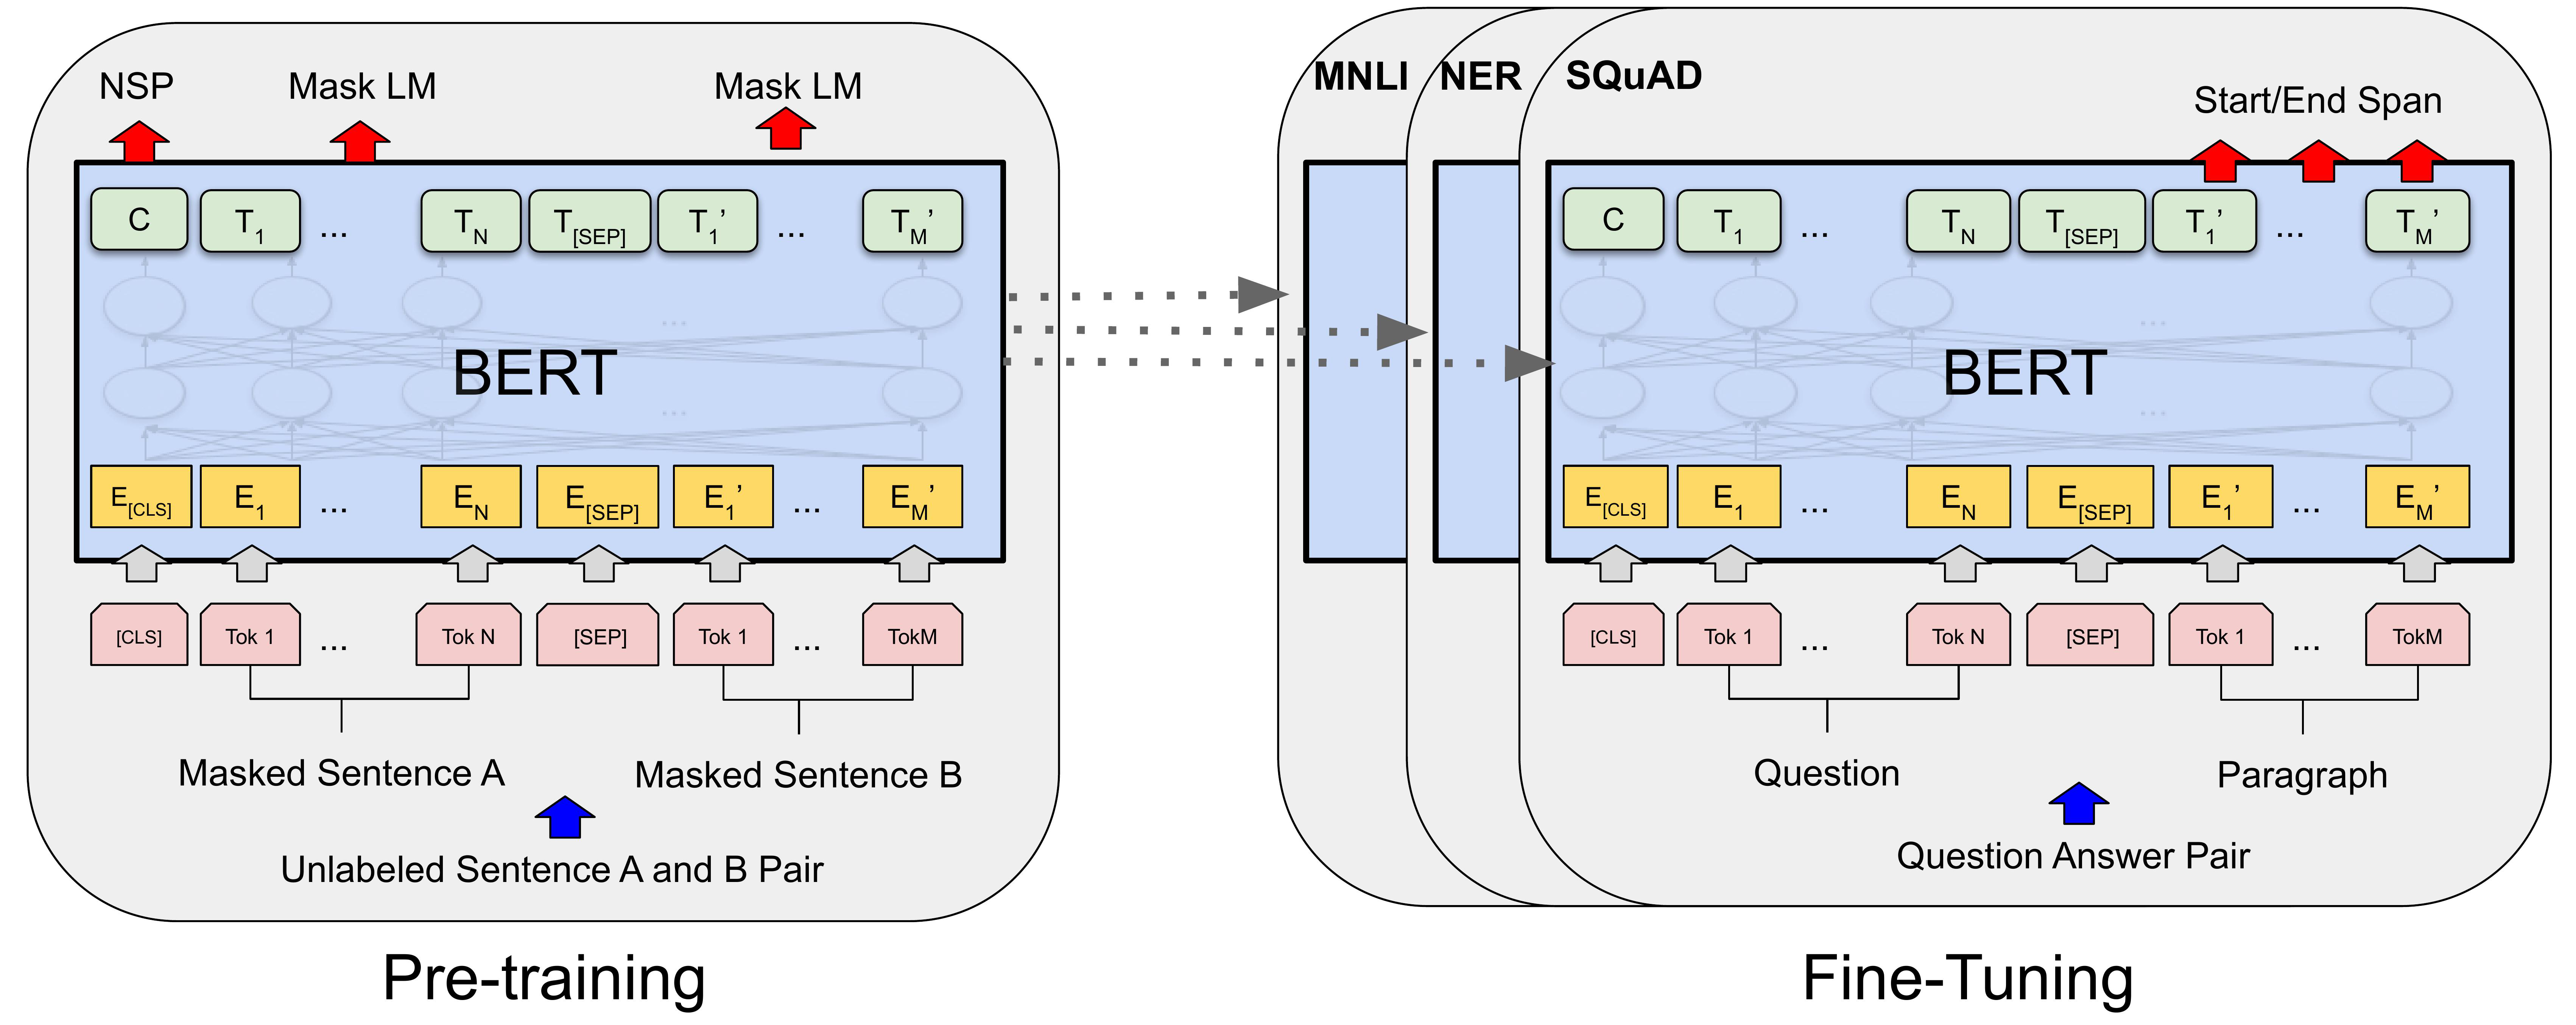
\includegraphics[width=\textwidth]{chapter-2/bert.jpg}
    \caption{Arsitektur BERT \parencite{bert}}
    \label{fig:bert}
\end{figure}

BERT merupakan \textit{pre-trained model} sehingga telah dilatih pada sejumlah besar teks. Data latih BERT diambil dari BooksCorpus dan Wikipedia bahasa Inggris \parencite{bert}. Ini memungkinkan BERT untuk mempunyai pengetahuan mendasar dalam tugas NLP. Ketika digunakan untuk tugas-tugas NLP spesifik, seperti klasifikasi teks atau pemahaman pertanyaan, BERT dapat disesuaikan dengan data tugas spesifik untuk meningkatkan kinerjanya. Seperti yang bisa dilihat pada gambar \ref{fig:bert}, BERT dilatih (\textit{pre-train}) dengan menggunakan dua tugas yaitu \textit{Masked LM} dan \textit{Next Sentence Prediction} (NSP). \textit{Masked LM} melakukan \textit{masking} pada sebagian token dan akan diprediksi oleh model BERT. Sedangkan, untuk NSP, model BERT akan menentukan mana kalimat berikutnya dari kalimat sebelumnya.

Terdapat versi bahasa Indonesia yaitu IndoBERT. IndoBERT merupakan model Transformer yang mirip dengan BERT, namun dilatih dengan bahasa Indonesia \parencite{indolem}. IndoBERT mempunyai konfigurasi yang sama dengan konfigurasi BERT, yaitu 12 \textit{layer} yang masing-masing mempunyai 768 \textit{hidden layer}, 12 \textit{attention head}, dan 3072 \textit{hidden layer} pada \textit{feed-forward layer}. IndoBERT dilatih dengan total 220 juta kata, yang didapatkan dari tiga sumber utama, yaitu Wikipedia Indonesia, sumber berita (Kompas, Tempo, dan Liputan6), dan Indonesian Web Corpus \parencite{indolem}. IndoBERT merupakan \textit{state-of-the-art} pada kakas evaluasi IndoLEM.

\subsection{\textit{Text-to-Text Transfer Transformers} (T5)}

\textit{Text-to-Text Transfer Transformers} atau biasa disebut sebagai T5 merupakan model \textit{encoder decoder} berbasis Transformer. Model ini menggunakan pendekatan \textit{text-to-text} seperti namanya, yang berarti menganggap setiap pemrosesan teks sebagai masukan dan mengeluarkannya sebagai teks juga \parencite{T5}. Dengan pendekatan ini, model T5 dapat digunakan secara langsung pada setiap tugas NLP.

\begin{figure}[ht]
    \vspace{0.25cm}
    \centering
    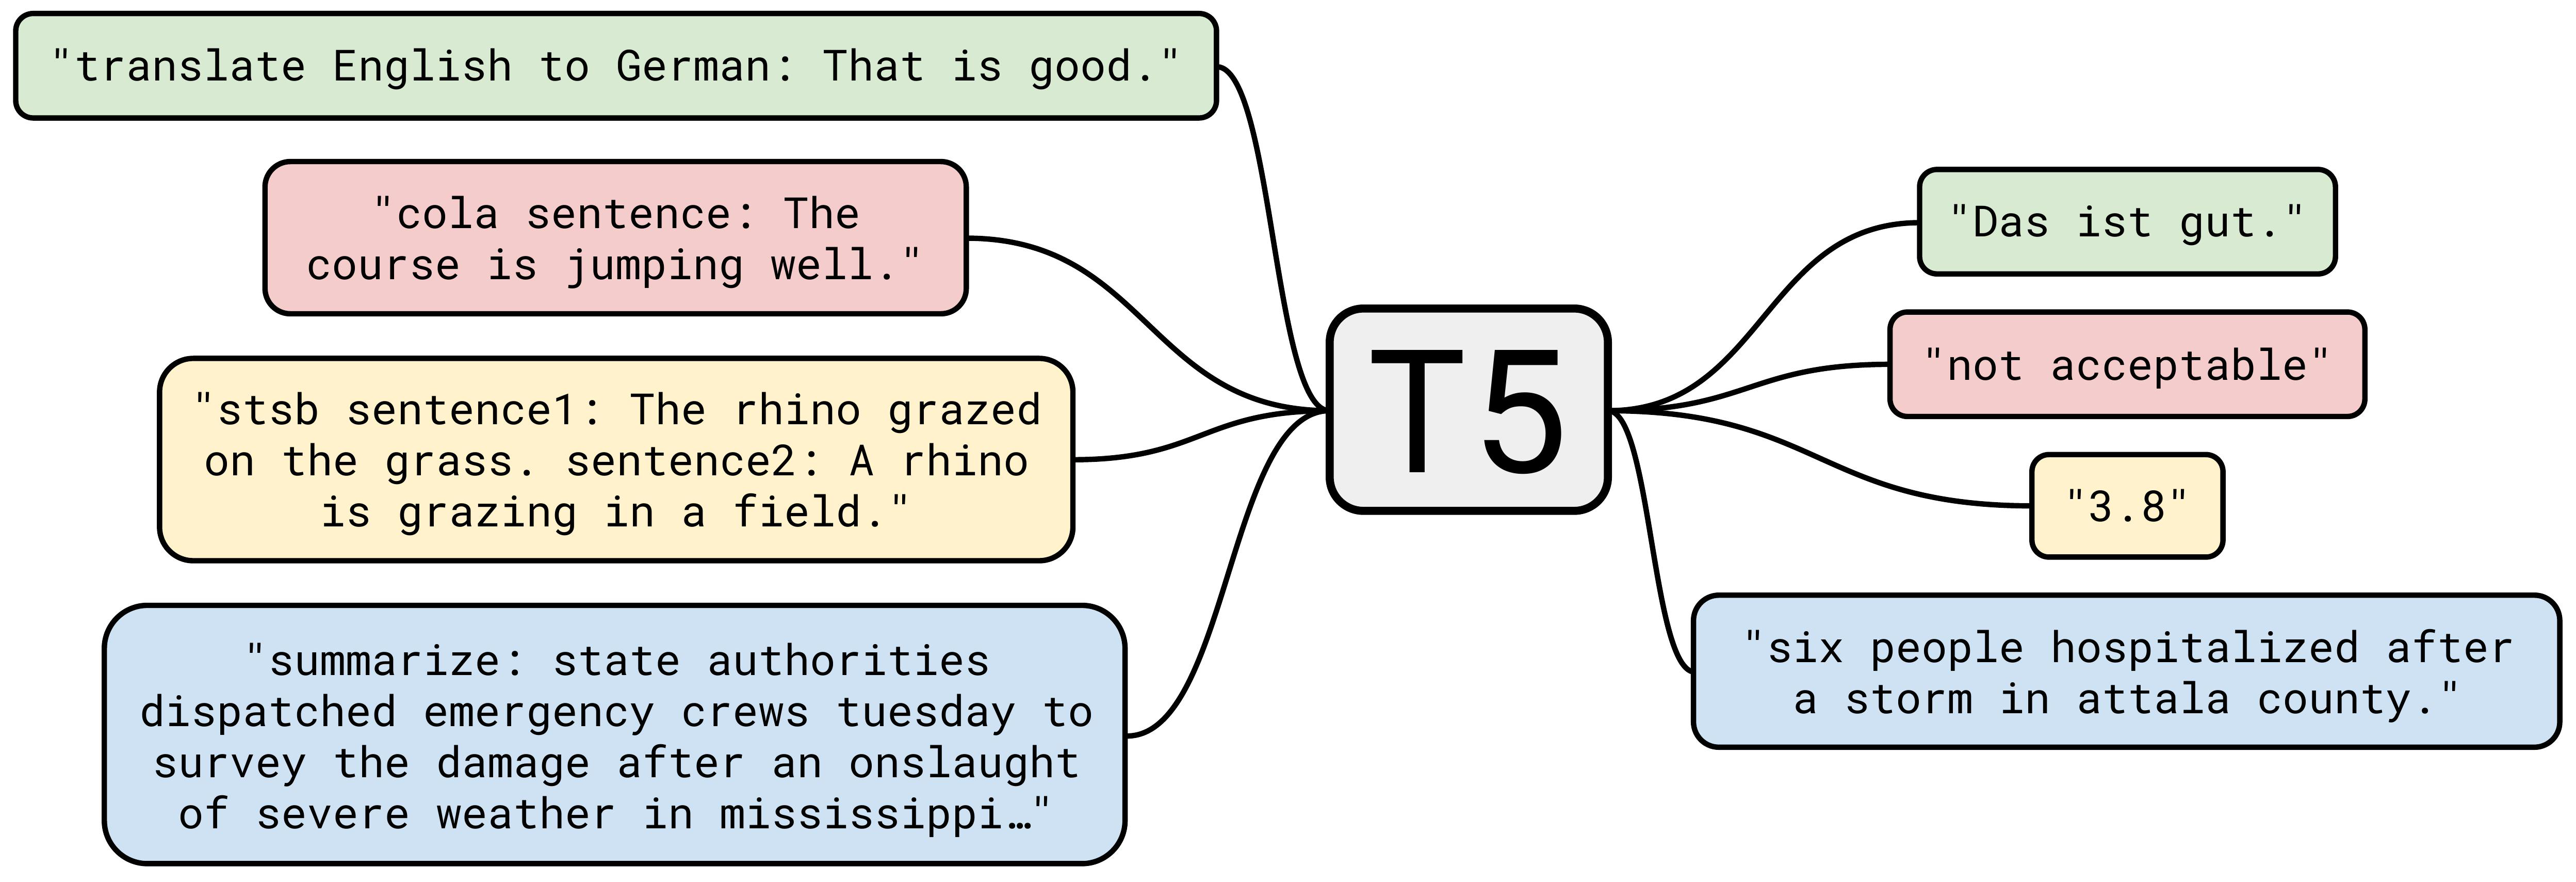
\includegraphics[width=\textwidth]{chapter-2/T5.jpg}
    \caption{\textit{Framework} dari T5 \parencite{T5}}
    \label{fig:T5}
\end{figure}

Pada gambar \ref{fig:T5}, yaitu \textit{framework} dari model T5, setiap tugas pada T5, termasuk \textit{translation, question answering}, dan \textit{classification}, semuanya akan dianggap sebagai masukan teks dan dilatih untuk menghasilkan teks lainnya lagi. T5 dilatih pada dataset \textit{Colossal Cleaned Crawled Corpus} (C4) yang merupakan koleksi dari web publik Common Crawl yang telah dibersihkan.

\begin{figure}[ht]
    \vspace{0.25cm}
    \centering
    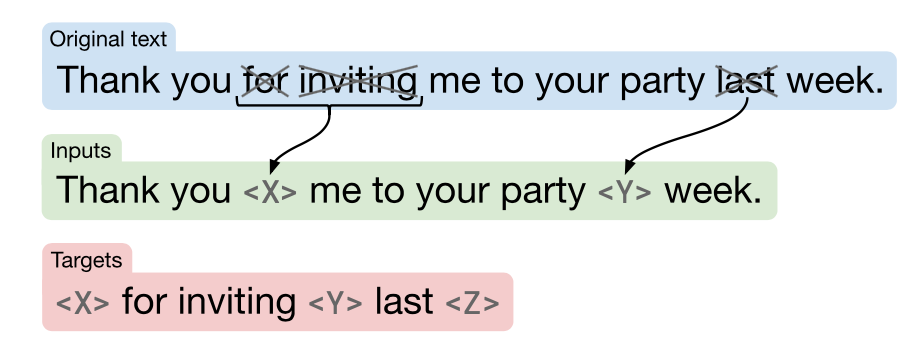
\includegraphics[width=\textwidth]{chapter-2/unsupervised_objective.png}
    \caption{\textit{Unsupervised objectives} dari T5 \parencite{T5}}
    \label{fig:unsupervised-T5}
\end{figure}

Model T5 didesain agar bagian \textit{encoder} dan \textit{decoder}-nya mirip dengan konfigurasi dari BERT \parencite{T5}. Kedua bagian tersebut terdiri dari 12 \textit{layer} yang mempunyai \textit{hidden layer, attention head}, serta \textit{feed-forward}. Mirip dengan MLLM pada BERT, model T5 dilatih \textit{pre-train} dengan menggunakan \textit{unsupervised objectives} yang bisa dilihat pada gambar \ref{fig:unsupervised-T5}. Beberapa kata yang dihilangkan secara konsekutif akan dianggap sebagai satu \textit{sentinel} token yang nantinya akan diprediksi sebagai target oleh T5.

Terdapat versi bahasa Indonesia dari T5, yaitu IndoT5. IndoT5 dilatih secara spesifik untuk bahasa Indonesia dengan menggunakan \textit{framework} pelatihan nanoT5 \parencite{indoT5}. \textit{Dataset} yang digunakan berasal dari CulturaX yang mengandung 23 juta dokumen berbahasa Indonesia. Model IndoT5 menjadi \textit{state-of-the-art} pada tugas \textit{summarization} pada kakas evaluasi IndoLEM.

\subsection{\textit{Bidirectional Encoder Representations from Transformers} \\ (BERT)}

BERT, yang merupakan singkatan dari \textit{Bidirectional Encoder Representations from Transformers}, adalah model pemrosesan bahasa alami yang diperkenalkan oleh Google pada tahun 2018 \parencite{bert}. BERT memanfaatkan arsitektur \textit{transformer}, yang telah dibahas sebelumnya, untuk memahami konteks kata dalam teks dengan cara yang lebih mendalam daripada pendekatan sebelumnya.

BERT menggunakan pendekatan yang \textit{bidirectional}. BERT mampu memahami teks dari kiri ke kanan atau sebaliknya, BERT memahami konteks kata dengan mempertimbangkan informasi dari kedua arah. Sehingga, model ini memiliki kemampuan untuk pemahaman yang lebih kaya tentang makna dan nuansa dalam teks.

\begin{figure}[ht]
    \centering
    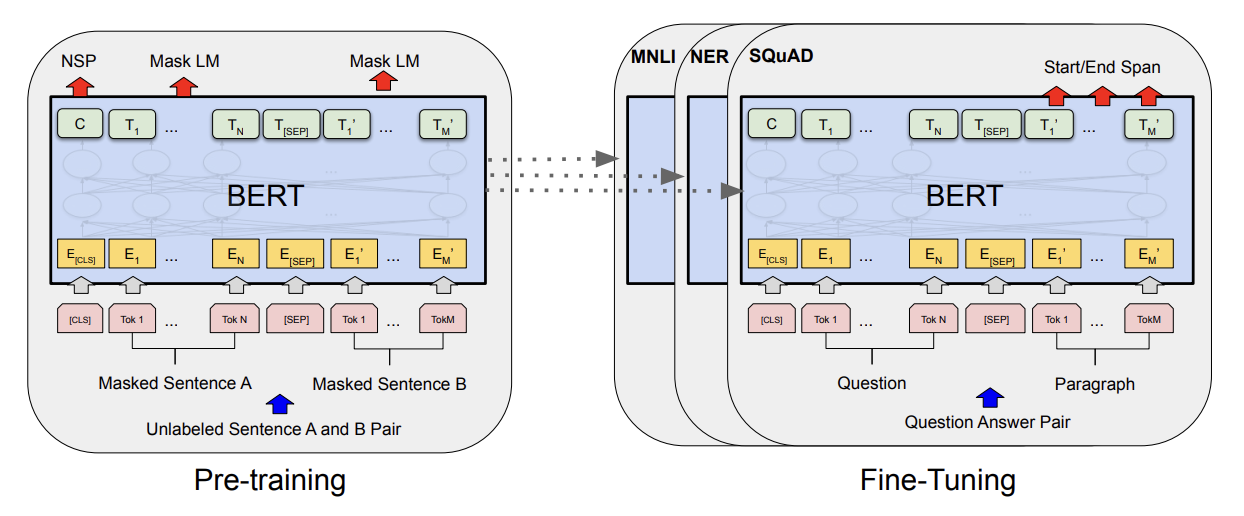
\includegraphics[width=0.8\textwidth]{chapter-2/bert.png}
    \caption{Arsitektur \textit{BERT} \parencite{bert}}
    \label{fig:bert}
\end{figure}

BERT merupakan \textit{pre-trained model} sehingga telah dilatih pada sejumlah besar teks. Data latih BERT diambil dari BooksCorpus dan Wikipedia bahasa Inggris. Ini memungkinan BERT untuk mempunyai pengetahuan mendasar dalam tugas NLP. Ketika digunakan untuk tugas-tugas NLP spesifik, seperti klasifikasi teks atau pemahaman pertanyaan, BERT dapat disesuaikan dengan data tugas spesifik untuk meningkatkan kinerjanya.

Model ini dikembangkan dengan dua konfigurasi, yaitu BASE dan LARGE. BERT dengan konfigurasi BASE memiliki 12 \textit{layer encoder} yang mempunyai 768 \textit{hidden layer} pada FFNN dan 12 \textit{attention heads}. Sedangkan, untuk konfigurasi BERT LARGE memiliki 24 \textit{layer encoder} yang mempunyai 1024 \textit{hidden layer} pada FFNN dan 16 \textit{attention heads}.
\subsection{IndoBERT}
\label{sec:indobet}

Meskipun terdapat lebih dari 200 juta pengguna bahasa Indonesia, bahasa tersebut kurang terwakili di NLP \parencite{indolem}. Sehingga, IndoBERT muncul untuk memperbaiki situasi ini. IndoBERT adalah adaptasi dari model BERT yang khusus dilatih untuk bahasa Indonesia. Mengingat keunikan dan kompleksitas bahasa Indonesia, memiliki model yang khusus dilatih untuk bahasa ini sangat penting untuk memastikan kinerja yang optimal pada tugas-tugas NLP yang berfokus pada bahasa Indonesia \parencite{indolem}.

\begin{figure}[ht]
    \centering
    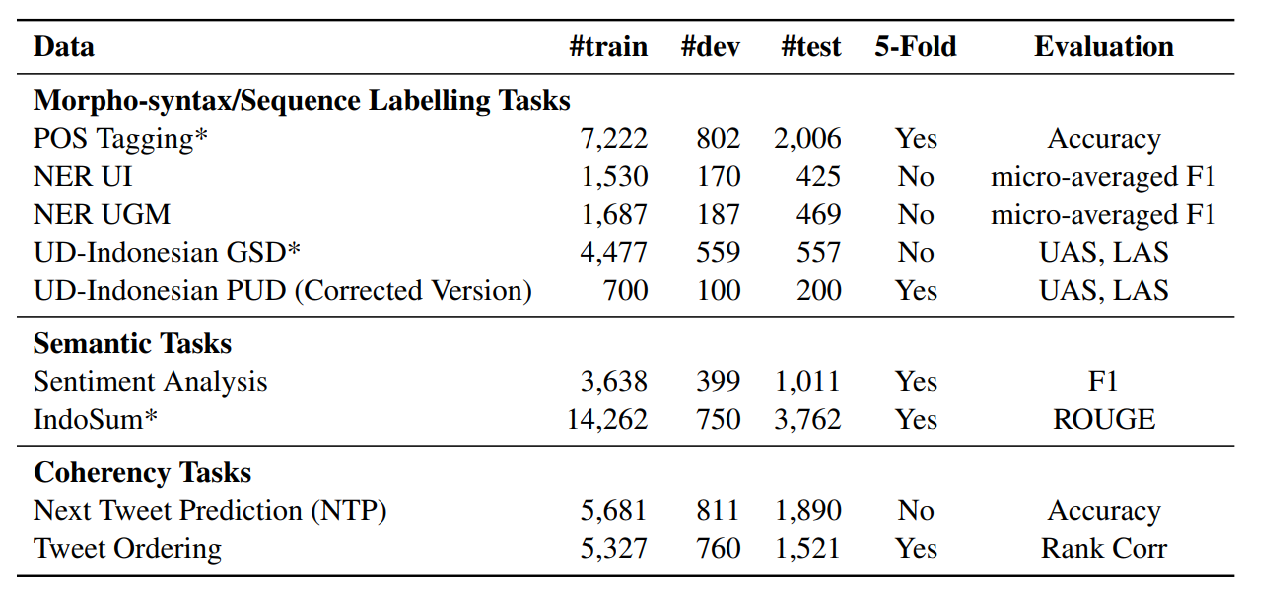
\includegraphics[width=0.8\textwidth]{chapter-2/indobert_dataset.png}
    \caption{\textit{Dataset} pada IndoBERT \parencite{indolem}}
    \label{fig:indobert_dataset}
\end{figure}

IndoBERT berbasis pada \textit{pre-trained model} BERT yang dilatih secara khusus pada \textit{dataset} berbahasa Indonesia, seperti yang bisa dilihat pada Gambar \ref{fig:indobert_dataset}. Tugas NLP yang dilatih pada IndoBERT dibagi menjadi tiga, yaitu \textit{sequence labelling}, \textit{semantic}, dan \textit{coherency}. Untuk \textit{sequence labelling} terdapat tiga tugas, yaitu \textit{part-of-speech} (POS) \textit{tagging}, \textit{named entity recognition} (NER), dan \textit{dependency parsing}. Lalu, untuk \textit{semantic} terdapat dua tugas, yaitu \textit{sentiment analysis} dan \textit{summarization}. Terakhir, untuk \textit{coherency} terdapat dua tugas, yaitu \textit{next tweet prediction} dan \textit{tweet ordering}.

\begin{figure}[ht]
    \centering
    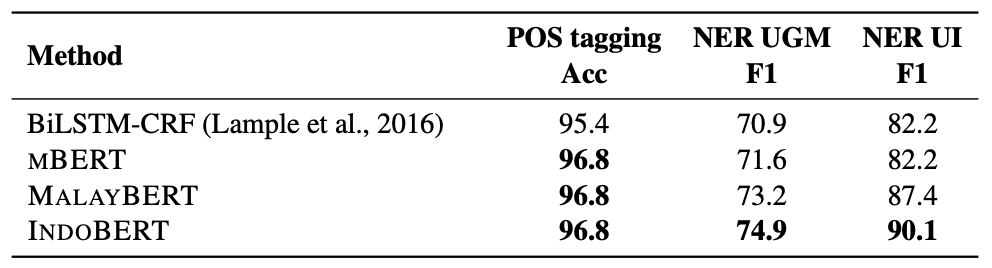
\includegraphics[width=0.8\textwidth]{chapter-2/indobert_pos.png}
    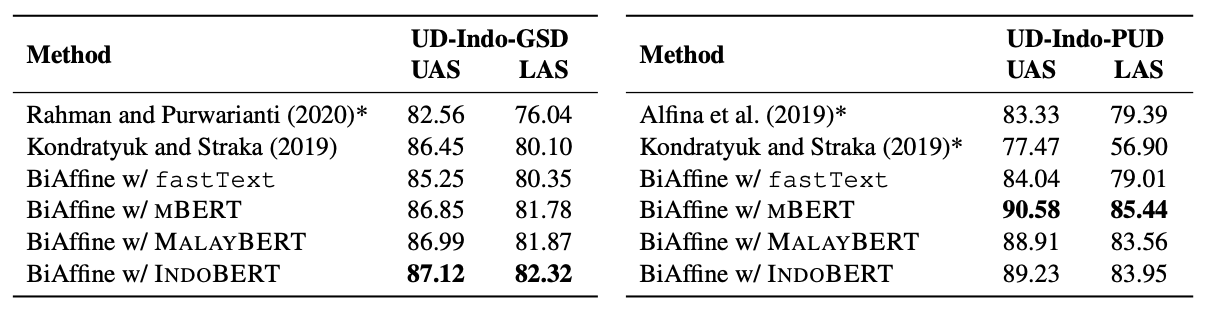
\includegraphics[width=0.8\textwidth]{chapter-2/indobert_dependency_parsing.png}
    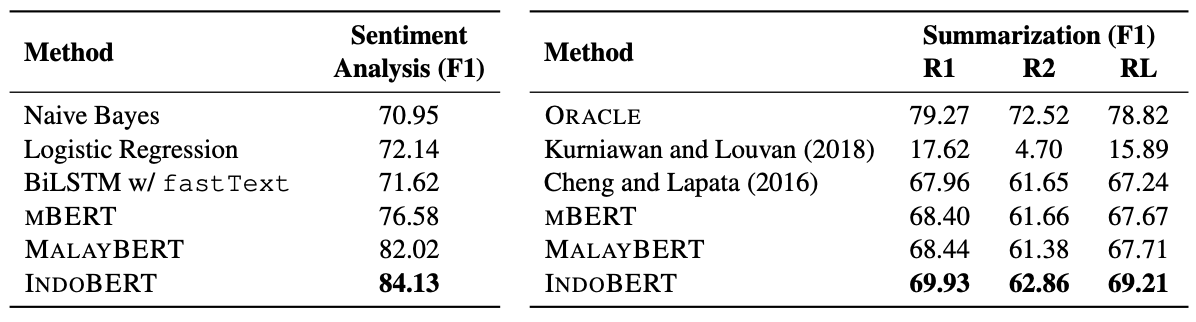
\includegraphics[width=0.8\textwidth]{chapter-2/indobert_semantic.png}
    \caption{Hasil Evaluasi IndoBERT \parencite{indolem}}
    \label{fig:indobert_evaluation}
\end{figure}

Untuk melakukan evaluasi terhadap model, dilakukan perbandingan dengan model lain. Pada penelitian ini, digunakan \textit{multilingual} BERT (mBERT) dan MalayBERT yang di-\textit{fine-tune} dengan bahasa Indonesia sebagai pembanding \parencite{indolem}. Hasilnya, IndoBERT kebanyakan unggul di setiap tugas. Selain dari tugas \textit{part-of-speech} (POS) \textit{tagging} dan \textit{next-tweet prediction} masih bisa dilakukan peningkatan \parencite{indolem}. Hasil evaluasi secara detail dapat dilihat pada Gambar \ref{fig:indobert_evaluation}.


\section{\textit{Transfer Learning}}

\textit{Transfer Learning} merupakan salah satu pendekatan kunci dalam pembelajaran mesin yang memanfaatkan model yang telah dilatih pada tugas tertentu sebagai dasar untuk melatih model pada tugas lain. Ide dasar di balik \textit{transfer learning} adalah bahwa, jika model telah mempelajari fitur-fitur tertentu dari satu tugas, fitur-fitur tersebut dapat digunakan sebagai informasi awal yang berguna untuk tugas lain.

Sebagai contoh, model yang telah dilatih untuk mengenali objek dalam gambar dapat memanfaatkan pengetahuannya tentang fitur visual, seperti tepi atau tekstur, saat dilatih untuk tugas pengenalan wajah. Meskipun tugas awal (mengenali objek) dan tugas kedua (pengenalan wajah) berbeda, ada sejumlah fitur visual yang relevan untuk kedua tugas tersebut.

Dalam konteks pemrosesan bahasa alami (NLP), \textit{transfer learning} sering digunakan untuk memanfaatkan \textit{Pre-Trained Model} (PLM) yang telah dilatih pada korpus teks besar untuk tugas-tugas spesifik seperti \textit{sentiment analysis} atau \textit{named entity recognition}. Dengan memulai dari model yang telah memiliki pemahaman dasar tentang struktur dan semantik bahasa, proses \textit{training} untuk tugas spesifik menjadi lebih cepat dan seringkali menghasilkan model yang lebih akurat dibandingkan dengan melatih model dari awal.

Keuntungan lain dari \textit{transfer learning} adalah efisiensi komputasi. Melatih model pembelajaran mesin dari awal, terutama model dengan banyak parameter, memerlukan sumber daya komputasi yang signifikan. Dengan menggunakan model yang telah dilatih sebagai titik awal, dapat menghemat waktu dan sumber daya komputasi, sambil mempertahankan atau bahkan meningkatkan kinerja model.


\subsection{\textit{Low Rank Adaptation} (LoRA)}

Dalam dunia pembelajaran mesin, terutama saat bekerja dengan model berukuran besar, efisiensi parameter menjadi salah satu tantangan utama. LoRA, singkatan dari \textit{Low Rank Adaptation}, muncul sebagai solusi untuk tantangan ini dalam konteks \textit{transfer learning}.

Konsep dasar di balik LoRA adalah ide bahwa adaptasi model untuk tugas baru tidak selalu memerlukan perubahan besar pada seluruh parameter model. Sebaliknya, perubahan kecil pada representasi tertentu dapat menghasilkan peningkatan kinerja yang signifikan. Dengan fokus pada adaptasi peringkat rendah, LoRA mengubah hanya sebagian kecil dari bobot model, sementara sebagian besar bobot lainnya tetap tidak berubah. Ini berarti bahwa hanya "sebagian" dari informasi dalam model yang diperbarui, yang mengarah pada efisiensi komputasi yang meningkat \parencite{lora}.

Salah satu kelebihan utama dari pendekatan ini adalah kemampuannya untuk mengurangi overhead komputasi. Dalam praktiknya, ini berarti bahwa waktu pelatihan dan sumber daya yang diperlukan untuk adaptasi model menjadi jauh lebih sedikit dibandingkan dengan metode lain yang mungkin melibatkan pelatihan ulang model dari awal atau menambahkan sejumlah besar parameter tambahan.

Pendekatan LoRA menjadi sangat relevan dan berharga, terutama saat berhadapan dengan model-model berukuran besar seperti GPT-3. Model-model seperti ini memiliki jumlah parameter yang sangat besar, sehingga pelatihan ulang atau menambahkan parameter tambahan bisa menjadi sangat mahal dari segi komputasi. Dengan LoRA, adaptasi model-model besar menjadi lebih praktis dan dapat dilakukan dengan efisiensi yang jauh lebih tinggi, tanpa mengorbankan kinerja.

Dengan demikian, LoRA menawarkan pendekatan yang menjanjikan untuk mengadaptasi model pra-latih dengan cara yang lebih efisien, memungkinkan peneliti dan praktisi untuk memanfaatkan kekuatan model berukuran besar tanpa harus berurusan dengan beban komputasi yang berat.
\subsection{\textit{Prefix-Tuning}}

\textit{Prefix-Tuning} adalah teknik yang diperkenalkan untuk mengoptimalkan prompt kontinu dalam generasi teks. Berbeda dengan pendekatan tradisional yang melibatkan \textit{training} ulang seluruh model atau menambahkan parameter tambahan, \textit{Prefix-Tuning} fokus pada pengoptimalan sejumlah kecil parameter yang didefinisikan sebagai "prefix" dari sekuens input \parencite{prefix_tuning}. Dengan kata lain, alih-alih mengubah seluruh model, hanya \textit{prefix} dari input yang dioptimalkan untuk meningkatkan kinerja generasi.

\begin{figure}[ht]
    \centering
    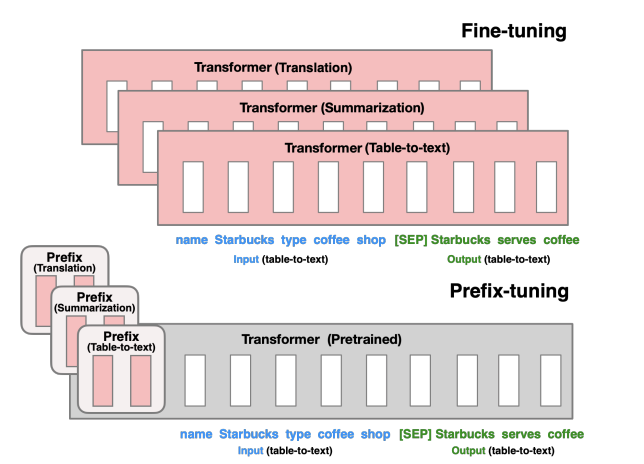
\includegraphics[width=0.8\textwidth]{chapter-2/prefix-tuning.png}
    \caption{Arsitektur \textit{Prefix-Tuning} \parencite{prefix_tuning}}
    \label{fig:prefix-tuning}
\end{figure}

Keuntungan utama dari pendekatan ini adalah efisiensi. Dengan mengoptimalkan hanya sebagian kecil dari parameter, \textit{Prefix-Tuning} dapat mencapai peningkatan kinerja dengan \textit{overhead} komputasi yang jauh lebih rendah dibandingkan dengan teknik \textit{fine-tuning} tradisional. Selain itu, dengan fokus pada \textit{prefix}, teknik ini memungkinkan adaptasi yang lebih spesifik terhadap tugas atau domain tertentu, memberikan fleksibilitas lebih dalam aplikasi praktis.

Teknik ini dapat digunakan untuk meningkatkan kinerja model generatif di berbagai tugas, termasuk penerjemahan mesin, peringkasan teks, dan lainnya. Hasil eksperimen menunjukkan bahwa \textit{Prefix-Tuning} mampu mencapai kinerja yang sebanding atau bahkan lebih baik dibandingkan dengan metode \textit{fine-tuning} tradisional, tetapi dengan biaya komputasi yang jauh lebih rendah.


\subsection{\textit{Tiny Attention Adapter}}

\textit{Tiny-Attention Adapter} merupakan salah satu solusi yang dirancang untuk mengatasi waktu komputasi. Sebagai gantinya dari menambahkan lapisan adaptasi berukuran besar atau melatih ulang seluruh model, teknik ini memperkenalkan konsep "\textit{tiny-attention}". Mekanisme ini, meskipun sederhana, memungkinkan setiap posisi dalam sekuens untuk memperhatikan dan memodifikasi keadaan tersembunyinya berdasarkan informasi dari semua posisi lain dalam sekuens \parencite{tinyattention}. Dengan kata lain, setiap elemen dalam sekuens memiliki kemampuan untuk "berkomunikasi" dan "berkoordinasi" dengan elemen lain untuk membentuk representasi yang lebih kaya dan kontekstual.

Salah satu kelebihan dari pendekatan ini adalah fleksibilitas dan dinamikanya. Karena setiap posisi dapat memperhatikan semua posisi lain, model memiliki kapasitas untuk memahami hubungan antar kata dengan lebih baik, terutama hubungan yang bersifat jarak jauh atau kontekstual yang kompleks. Ini memungkinkan model untuk menangkap nuansa dan makna yang mungkin terlewatkan oleh teknik adaptasi lainnya.

\begin{figure}[ht]
    \centering
    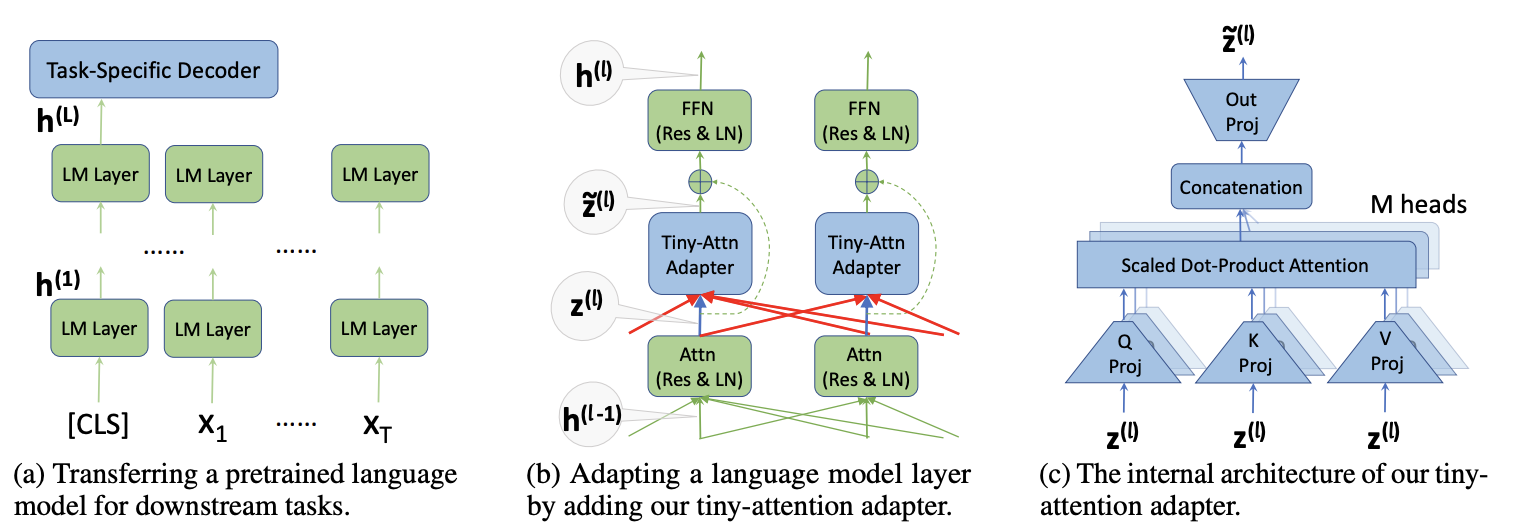
\includegraphics[width=0.8\textwidth]{chapter-2/tiny-attention.png}
    \caption{Arsitektur \textit{Tiny-Attention Adapter}}
    \label{fig:tiny-attention}
\end{figure}


Meskipun pendekatan ini terfokus pada efisiensi parameter, \textit{Tiny-Attention Adapter} tidak mengorbankan kinerja. Sebaliknya, berkat mekanisme "tiny-attention", teknik ini seringkali mampu mencapai kinerja yang sebanding atau bahkan melampaui metode adaptasi tradisional, meskipun hanya dengan sebagian kecil dari parameter tambahan.

Dengan demikian, \textit{Tiny-Attention Adapter} menawarkan pendekatan yang menjanjikan untuk mengadaptasi \textit{pre-trained model} dengan cara yang lebih efisien, tanpa mengorbankan kualitas atau kinerja.

\section{Metriks Evaluasi}

Dalam proses \textit{training} model, diperlukan metode evaluasi sebagai penilaian kinerja model dengan membandingkan metriks yang dihasilkan oleh model tersebut. Metriks ini digunakan pada model klasifikasi dengan membandingkan hasil prediksi dengan target aslinya. Hasil prediksi ini dapat direpresentasikan sebagai \textit{confusion matrix}. Berdasarkan \citeauthor{metrics}, terdapat beberapa metriks yang dapat dihasilkan berdasarkan \textit{confusion matrix}, yaitu \textit{accuracy}, \textit{precision}, \textit{recall}, dan F1-\textit{Score}.

\begin{table}[ht]
\centering
\caption{\textit{Confusion matrix}}
\label{confusion-matrix}
\begin{tabular}{|l|c|c|}
\hline
\rowcolor{black!10}
\multicolumn{1}{|c|}{\textbf{Target}} & \multicolumn{2}{c|}{\textbf{Prediksi}} \\ \cline{2-3} 
\rowcolor{black!10}
& \textbf{Positif} & \textbf{Negatif} \\ \hline
\textbf{Positif} & \textit{True Positive} (TP) & \textit{False Negative} (FN) \\ \hline
\textbf{Negatif} & \textit{False Positive} (FP) & \textit{True Negative} (TN) \\ \hline
\end{tabular}
\end{table}

Berdasarkan tabel \ref{confusion-matrix} terdapat empat hasil prediksi. \textit{True Positive} (TP) yang berarti model memprediksi kelas positif yang memang bernilai positif sesuai kelasnya. True Negative (TN) memprediksi kelas negatif dan kelas tersebut memang bernilai negatif. Sedangkan, \textit{False Positive} (FP) me\textit{mprediksi kelas} positif, tetapi kelas tersebut bernilai negatif. Sebaliknya juga untuk \textit{False Negative} (FN) model memprediksi kelas tersebut sebagai negatif, tetapi kelas tersebut bernilai positif.

\subsection{\textit{Accuracy}}
Nilai \textit{accuracy} dihitung sebagai proporsi hasil prediksi yang benar (baik TP maupun TN) dari total jumlah prediksi. Metriks ini memberikan gambaran keseluruhan tentang keefektifan model. Dengan rumus sebagai berikut.

\begin{equation}
    Accuracy = \frac{TP + TN}{TP + TN + FP + FN}
\end{equation}

\subsection{\textit{Precision}}
Nilai \textit{precision} menilai proporsi prediksi positif yang benar-benar positif. Metriks ini memberikan gambaran tentang keakuratan model dalam memprediksi kelas positif. Dengan rumus sebagai berikut.
\begin{equation}
    Precision = \frac{TP}{TP + FP}
\end{equation}

\subsection{\textit{Recall}}
Nilai \textit{recall} menilai proporsi kasus positif sebenarnya yang berhasil diidentifikasi oleh model. Metrix Ini berfungsi untuk mengukur kemampuan model dalam mengidentifikasi semua kasus positif. Dengan rumus sebagai berikut.
\begin{equation}
    Recall = \frac{TP}{TP + FN}
\end{equation}

\subsection{F1-\textit{Score}}
Nilai F1-\textit{Score} direpresentasikan sebagai nilai rata-rata harmonis dari nilai \textit{precision} dan \textit{recall}. Metriks ini berfungsi untuk mengukur keseimbangan dari kedua metriks tersebut. Dengan rumus sebagai berikut.
\begin{equation}
    F1-Score = 2 \times \frac{Precision \times Recall}{Precision + Recall}
\end{equation}

\section{\textit{NLP Task Benchmarking}}

Dalam pemrosesan bahasa alami (NLP), pentingnya evaluasi kinerja model pada berbagai tugas tidak dapat diremehkan. Evaluasi memberikan cara standar untuk membandingkan berbagai model dan teknik dalam konteks aplikasi nyata.

\subsection{\textit{General Language Understanding Evaluation} (GLUE)}

GLUE, yang merupakan singkatan dari \textit{General Language Understanding Evaluation}, adalah inisiatif yang dirancang untuk memajukan pemahaman bahasa alami melalui evaluasi yang konsisten dan komprehensif \parencite{glue}. Dengan latar belakang yang semakin meningkatnya kompleksitas dan variasi model NLP, muncul kebutuhan untuk memiliki metrik evaluasi yang standar dan konsisten. 

Salah satu ciri khas dari GLUE adalah kumpulan tugas evaluasinya yang beragam. Ini mencakup tugas-tugas seperti analisis sentimen, dengan tujuannya adalah untuk menentukan apakah teks tertentu memiliki konotasi positif, negatif, atau netral; jawaban pertanyaan, dengan model diberi pertanyaan dan harus memilih jawaban yang paling tepat dari kumpulan pilihan; dan entailment teks, dengan model harus menentukan apakah satu kalimat secara logis mengikuti kalimat lain.

Namun, bukan hanya variasi tugas yang membuat GLUE menjadi penting. GLUE juga menyediakan papan peringkat, yang memungkinkan peneliti untuk membandingkan kinerja model mereka dengan model-model lain dalam kondisi yang sama. Selain itu, GLUE juga memberikan kesempatan bagi peneliti untuk memahami kelemahan dan kekuatan model mereka. Dengan memiliki berbagai tugas evaluasi, peneliti dapat melihat kelemahan dari model yang berguna untuk mengembangkan model.
\subsection{IndoLEM}
% TODO: jelasin proses eksperimen saat ini, dan datasetnya juga 
IndoLEM muncul sebagai respons terhadap kebutuhan industri dan komunitas penelitian untuk memiliki \textit{benchmark} yang khusus dirancang untuk mengevaluasi model NLP dalam konteks bahasa Indonesia \parencite{indolem}. Meskipun ada banyak \textit{benchmark} NLP yang tersedia, seperti GLUE, kebanyakan dari mereka berfokus pada bahasa Inggris. Namun, dengan keragaman linguistik yang kaya, bahasa Indonesia memerlukan pendekatan khusus dalam evaluasi model NLP.

IndoLEM tidak hanya menyediakan kumpulan tugas evaluasi yang dirancang khusus untuk bahasa Indonesia, tetapi juga memastikan bahwa tugas-tugas tersebut mencerminkan nuansa dan tantangan unik yang diasosiasikan dengan bahasa ini. Salah satu aspek penting dari IndoLEM adalah dataset yang digunakannya. Mengingat pentingnya data dalam \textit{training} dan evaluasi model NLP, IndoLEM memastikan bahwa dataset yang digunakan berasal dari sumber-sumber lokal yang relevan. Ini memastikan bahwa model yang dievaluasi dengan IndoLEM benar-benar diuji dalam konteks yang sesuai dengan penggunaan sebenarnya dalam kehidupan nyata.


\section{Penelitian Terkait}

Pada sub-bab ini, akan dibahas beberapa penelitian yang telah dilakukan terhadap penggunaan metode PETL pada \textit{pre-trained model}.
\subsection{\textit{Unified View of Parameter-Efficient Transfer Learning}}

\textit{Unified Parameter Transfer Learning} merupakan upaya untuk menggabungkan beberapa metode PETL menjadi satu kesatuan \textit{framework} \parencite{uvpl}. Dalam \textit{transfer learning}, ide utamanya adalah mengambil \textit{pre-trained model} dan menyesuaikannya untuk tugas yang berbeda. Namun, ada banyak cara untuk melakukan adaptasi ini, dan setiap metode memiliki karakteristiknya masing-masing. Beberapa teknik mungkin fokus pada penambahan lapisan adaptasi, sementara yang lain mungkin memprioritaskan modifikasi parameter tertentu dalam model.

Metode PETL lain telah berhasil mengubah atau menambahkan sedikit parameter untuk mendapatkan kinerja yang setara dengan \textit{fine-tuning} tradisional, tetapi hubungan antara metode tersebut tidak dimengerti secara baik \parencite{uvpl}. Selain itu, dicari juga elemen desain pada metode ini yang menjadi aspek penting pada kesuksesan metode terkait. \citeauthor{uvpl} pada penelitiannya ini, mencari hubungan antara tiap metode ini dengan mengupas arsitektur dari setiap metode terkait. Metode yang digunakan pada penelitian yang dilakukan oleh \citeauthor{uvpl} adalah LoRA, \textit{prefix-tuning}, dan \textit{adapter}.

\begin{figure}[ht]
    \centering
    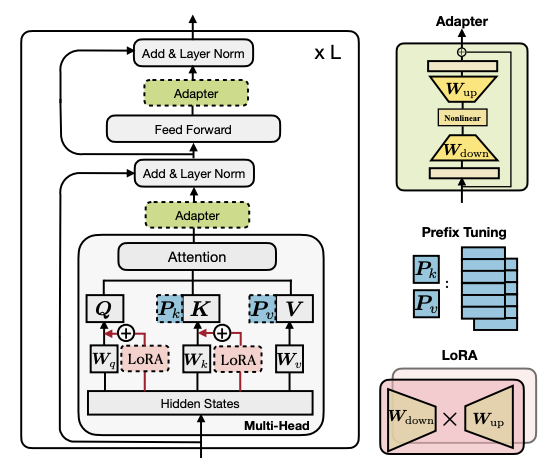
\includegraphics[width=0.8\textwidth]{chapter-2/uvpl.png}
    \caption{Arsitektur \textit{Unified View of Parameter-Efficient Transfer Learning} \parencite{uvpl}}
    \label{fig:uvpl}
\end{figure}

% TODO: tambahin secara jelas gimana tiap metode ini jadi satu dan hubungannya gimana
Arsitektur yang diajukan oleh \citeauthor{uvpl} pada penelitiannya dapat dilihat pada Gambar \ref{fig:uvpl}. Arsitektur tersebut menggabungan metode yang disebutkan sebelumnya pada model berbasis \textit{transformer}. 

\subsection{\textit{Parameter-Efficient Fine-Tuning of Large-Scale
Pre-Trained Language Models}}

Penelitian yang dilakukan oleh \citeauthor{peft_on_plm} membandingkan secara komprehensif terkait metode \textit{transfer-learning} yang efisien secara parameter pada \textit{pre-trained model}. Metode ini disebut sebagai \textit{delta-tuning} pada penelitian tersebut, dengan kata 'delta' muncul dari notasi matematika yang merepresentasikan perubahan \parencite{peft_on_plm}. Metode \textit{delta-tuning} yang digunakan adalah \textit{prompt-tuning} (PT), \textit{prefix-tuning} (PF), LoRA (LR), dan \textit{adapter} (AP). \textit{Delta-tuning} tersebut  dibandingkan dengan \textit{fine-tuning} (FT) .

Eksperimen yang dilakukan pada penelitian tersebut dilakukan pada model T5 dengan konfigurasi BASE dan LARGE. Evaluasi metode \textit{delta-tuning} pada model T5 dilakukan pada 100 tugas pemrosesan bahasa alami yang diambil dari \textit{dataset} Huggingface. Tugas yang dipilih termasuk \textit{text classification}, \textit{question answering}, dan \textit{generation}.

Berdasarkan hasil yang didapatkan pada eksperimen tersebut, metode \textit{delta-tuning} dengan pengurangan jumlah parameter yang dilatih dibandingkan dengan \textit{fine-tuning} memberikan hasil yang hampir setara pada sebagian besar tugas. Metode \textit{prefix-tuning}, LoRA, dan \textit{adapter} secara kinerja hampir mirip antara satu sama lain. Bahkan, metode \textit{delta-tuning} pada sebagian tugas mampu memberikan hasil yang dominan dibanding \textit{fine-tuning}. Secara keseluruhan, kinerja pada setiap metode dapat diurutkan sebagai berikut.

\begin{enumerate}
    \item \textit{Fine-Tuning} (FT)
    \item \textit{Low-Rank Adaptation} (LoRA)
    \item \textit{Adapter Tuning} (AP)
    \item \textit{Prefix Tuning} (PF)
    \item \textit{Prompt Tuning} (PT)
\end{enumerate}

Selain itu, dilakukan juga eksperimen terkait analisis pada efisiensi dari tiap metode. Eksperimen ini mengeksplorasi penggunaan efisiensi memori GPU pada metode \textit{delta-tuning} dan FT pada model T5 dengan konfigurasi BASE, LARGE, dan XL. Metode \textit{delta-tuning} yang digunakan adalah LoRA (LR), dan \textit{adapter} (AP), dan BitFit (BF). Berdasarkan Gambar \ref{fig:peft_on_plm_memory}, penggunaan memori pada setiap metode \textit{delta-tuning} berkurang dibandingkan dengan \textit{fine-tuning}. Hasil ini menunjukkan bahwa \textit{delta-tuning} mengurangi penggunaan memori GPU dengan mengurangi kebutuhan komputasi gradien untuk mengubah parameter.

\begin{figure}[ht]
    \centering
    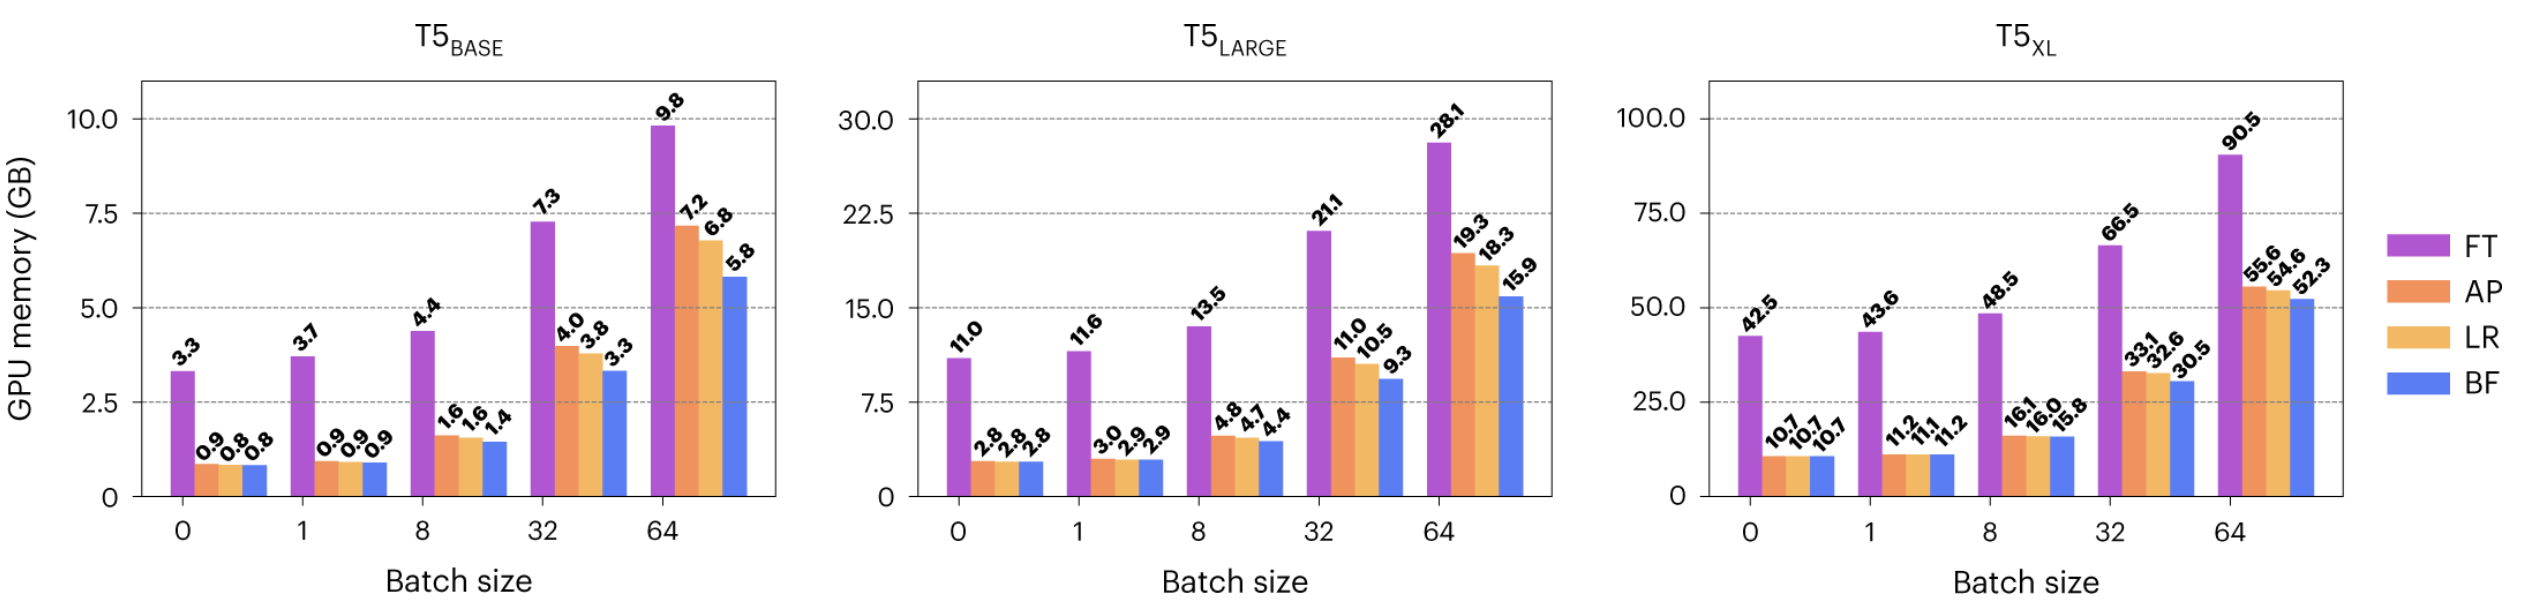
\includegraphics[width=1\textwidth]{chapter-2/peft_on_plm_memory.png}
    \caption{Perbandingan Efisiensi Memori \parencite{peft_on_plm}}
    \label{fig:peft_on_plm_memory}
\end{figure}

% \blankpage
\chapter{Analisis Persoalan dan Desain Eksperimen}
\label{sec:chapter-3}

Tujuan utama penulisan bab ini adalah untuk menguraikan rencana penyelesaian masalah tugas akhir sebelum dieksekusi. Bagian ini  memaparkan proses analisis masalah hingga menjadi solusi.

\section{Analisis Persoalan}
\label{sec:analisis-persoalan}

Berdasarkan latar belakang yang telah diuraikan pada subbab \ref{sec:latar-belakang}, peningkatan kinerja model IndoBERT dilakukan dengan menggunkan metode \textit{parameter-efficient transfer learning} (PETL). Peningkatan kinerja model dengan metode PETL ini melibatkan penambahan konfigurasi ataupun \textit{layer} tambahan terhadap model tergantung dengan karateristik dari metode PETL masing-masing. Untuk setiap metode PETL dibutuhkan \textit{dataset} tersendiri agar model dapat dilakukan \textit{transfer learning}. Selain itu, analisis komprehensif dibutuhkan untuk membandingkan metode PETL yang dapat memberikan hasil terbaik. Untuk membuat analisis yang komprehensif dibutuhkan metode evaluasi terhadap kinerja model. Secara keseluruhan, penelitian yang dilakukan pada tugas akhir ini akan mencakup tiga tahap sebagai berikut.

\begin{enumerate}
    \item Pengembangan dan konfigurasi pada setiap metode PETL.
    \item Integrasi model dengan \textit{dataset} yang dipilih.
    \item Eksperimen dan evaluasi kinerja model.
\end{enumerate}

Berdasarkan tahapan-tahapan penelitian yang diuraikan tersebut, terdapat empat persoalan utama dengan rincian sebagai berikut.

\begin{enumerate}
    \item Pemilihan \textit{dataset} yang sesuai untuk setiap tugas NLP.
    
    Berdasarkan tahap penelitian nomor 2 yaitu integrasi model dengan \textit{dataset} yang dipilih, diperlukan pencarian \textit{dataset} terlebih dahulu. Metode \textit{transfer learning} membutuhkan data yang relevan dengan tugas yang ingin dilatih. Diperlukan penilaian terhadap konten \textit{dataset} untuk memastikan kesesuaiannya dengan tugas NLP yang ditargetkan. Selain itu, kualitas \textit{dataset}, termasuk keakuratan label dan kebersihan data, serta ukurannya, harus cukup untuk memungkinkan model belajar secara efektif. Sehingga, pemilihan \textit{dataset} penting dilakukan untuk mendapatkan kinerja yang baik.

    \item Pemilihan konfigurasi terbaik untuk setiap metode PETL.
    
    Setiap metode PETL mempunyai karakteristik yang berbeda dalam penggunaannya, sehingga konfigurasi untuk setiap metode perlu diperhatikan. Proses ini melibatkan penyesuaian \textit{layer} dan parameter yang spesifik untuk setiap metode. Penting untuk mengeksplorasi berbagai konfigurasi untuk menemukan kombinasi yang paling efektif. Hal ini mencakup penyesuaian ukuran \textit{layer}, jumlah parameter, dan aspek teknis lainnya yang dapat mempengaruhi kinerja model. Selain itu, metode PETL juga memerlukan penambahan \textit{adapter} seperti pada teknik \textit{tiny-attention adapter}. Bahkan, menggabungkan beberapa metode PETL juga memungkinkan, sehingga diperlukan pembuatan konfigurasi yang spesifik untuk setiap metode.


    \item Pemilihan kombinasi \textit{hyperparameter} terbaik pada proses \textit{training}.
    
    Berdasarkan tahap penelitian nomor 3 yaitu eksperimen dan evaluasi kinerja model, proses \textit{transfer learning} melibatkan proses \textit{training}. Pada proses tersebut perlu pemilihan kombinasi \textit{hyperparameter} yang optimal. \textit{Hyperparameter} seperti \textit{learning rate}, \textit{batch size}, dan jumlah \textit{epoch} berperan penting dalam menentukan kinerja model. Proses ini melibatkan eksperimen dengan berbagai kombinasi untuk menemukan setelan yang memberikan hasil terbaik. 
    
    \item Pemilihan metode evaluasi
    
    Untuk dapat melakukan analisis terhadap model diperlukan adanya metode evaluasi yang memang relevan dengan tugas NLP-nya. Metode evaluasi yang digunakan pada proses \textit{training} berupa metrik seperti akurasi, \textit{presisi}, \textit{recall}, dan F1-\textit{score}. Sedangkan, untuk analisis komprehensif yang dilakukan terakhir akan digunakan IndoLEM sebagai \textit{NLP Task Benchmarking}

\end{enumerate}
\section{Analisis Solusi}

Berdasarkan analisis masalah, terdapat beberapa solusi yang dapat langsung menjawab permasalahan yang diuraikan pada Bab \ref{sec:analisis-persoalan}. Diajukan solusi-solusi yang dijabarkan pada analisis solusi berikut. Setiap bagian dari analisis solusi ini  menjawab setiap bagian pada analisis persoalan.

\subsection{Kakas IndoLEM yang \textit{Outdated}}

Untuk menjawab persoalaan ini, diperlukan pengembangan ulang untuk memperbarui dan memperbaiki infrastruktur dari kakas IndoLEM. Selain itu, proses ini juga diperlukan untuk mengembangkan metode PEFT karena metode tersebut memerlukan versi yang lebih baru dari pustaka yang digunakan. Untuk melakukan pengembangan ulang, terdapat beberapa langkah yang diperlukan, yaitu memperbarui versi dari perangkat lunak yang digunakan, penyederhanaan dan standardisasi proses, serta dokumentasi.

Peningkatan versi perangkat lunak yaitu Python ke versi lebih baru yang kompatibel dengan pustaka yang  digunakan beserta dependensinya, salah satunya adalah Torch dan Transformers. Hal ini perlu dilakukan karena versi pustaka yang digunakan pada kakas IndoLEM banyak yang tidak bisa digunakan pada versi Python yang lebih baru.

\textit{Script} yang saat ini digunakan pada kakas IndoLEM cukup berbeda antar setiap tugas evaluasi. Padahal, untuk setiap tugas evaluasi, proses pelatihannya itu bisa distandardisasi. Dengan menggunakan modul Trainer dari pustaka Transformers, bagian pelatihan bisa distandardisasi. Hanya perlu menyesuaikan pada bagian praproses data dan perhitungan metriksnya.

Dokumentasi pada kakas IndoLEM saat ini cukup terbatas, terutama pada \textit{requirement} untuk versi Python dan pustaka yang digunakannya. Dengan menambahkan \textit{requirement} yang dibutuhkan untuk menajalankan proses pelatihan dan evaluasi dapat menjawab masalah ini.

\subsection{Implementasi Metode PEFT pada Kakas IndoLEM}

Metode PEFT yaitu \methodPEFT perlu diimplementasikan pada kakas IndoLEM. Implementasi dari setiap metode PEFT ini terdapat pada penelitian terkaitnya. Tetapi, sudah banyak kakas yang memungkinkan untuk menggunakan metode ini dengan mengintegrasikannya pada model. Hal ini dilakukan dengan menggunakan pustaka dari metode PEFT tersebut.

Terdapat beberapa pustaka yang sudah mengimplementasikan metode PEFT, ada yang hanya mengimplementasikan satu, beberapa, atau bahkan menggabungkan beberapa metode PEFT tersebut. Salah satunya adalah pustaka PEFT, OpenDelta, dan Adapters. Setiap pustaka tersebut mempunyai metode PEFT yang berbeda. Pustaka PEFT hanya mengimplementasikan metodenya saja tanpa ada fungsionalitas untuk menggabungkan beberapa metode PEFT. Sedangkan, OpenDelta dan Adapters mampu untuk melakukan penggubangan metode PEFT. Hanya saja, metode PEFT yang bisa digunakan pada pustaka OpenDelta dan Adapters lebih sedikit dibandingkan dengan pustaka PEFT.

Pada tugas akhir ini,  dilakukan implementasi pada metode PEFT yaitu \methodPEFT. Selain itu juga, dilakukan penggabungan antara ketiga metode tersebut. Sehingga, yang bisa menjadi pilihan adalah pustaka OpenDelta dan Adapters. Berdasarkan aktivitas dari \textit{soure code}-nya, pustaka Adapters, masih banyak dilakukan perubahan, sedangkan OpenDelta tidak ada perubahan dari sekitar setahun yang lalu. Sehingg, pustaka Adapters yang  digunakan untuk implementasi metode PEFT pada kakas IndoLEM.

\subsection{Pemilihan Model}

Pada penelitian yang menerbitkan kakas IndoLEM, diterbitkan juga sekaligus modelnya yaitu IndoBERT. Seperti yang disebtukan pada subbab \ref{sec:indobet}, model IndoBERT menjadi \textit{state-of-the-art} pada hasil evaluasi pada kakas IndoLEM. IndoBERT merupakan model \textit{encoder} yang cocok untuk tugas \textit{classification}, sehingga sesuai dengan tugas evaluasi NER dan \textit{sentiment analysis}. Namun, untuk tugas \textit{generation} yaitu \textit{summarization} yang membutuhkan model \textit{encoder decoder} bukan hal yang sesuai.

Tugas evaluasi \textit{summarization} pada kakas IndoLEM menggunakan model IndoBERT yang merupakan model \textit{encoder}. Hal ini bisa dilakukan dengan menjadikan model yang sama sebagai \textit{decoder}-nya juga, menjadikan 2 model IndoBERT sebagai \textit{encoder} dan \textit{decoder}. Terdapat model yang merupakan \textit{encoder decoder} yang lebih cocok untuk tugas evaluasi \textit{summarization} yaitu model BART dan T5. Untuk versi bahasa Indonesianya, terdapat model IndoBART dan IndoT5. Berdasarkan hasil evaluasi dari IndoBART dan IndoT5, model IndoT5 menghasilkan evaluasi yang lebih baik daripada IndoBART. 

\subsection{Pelatihan dan Evaluasi Model}

Terdapat beberapa komponen dalam pelatihan dan evaluasi model, yaitu \textit{dataset} (latih, evaluasi dan uji), \textit{hyperparameter} yang digunakan, dan lingkungan pelatihan. Pada kakas IndoLEM, untuk tugas evaluasi \nlptask sudah terdapat \textit{dataset} yang tersedia. \textit{Dataset} yang telah tersedia ini tetap digunakan, \textit{dataset} tersebut sudah terbagi dalam 5-\textit{fold}. Perubahan dilakukan untuk menyesuaikan format dan nama kolom  lebih sesuai.

\textit{Hyperparameter} yang digunakan ada dua, yaitu \textit{hyperparameter} pelatihan seperti \textit{learning rate}, dan \textit{hyperparameter} metode PEFT seperti \textit{rank} pada LoRA. Kedua \textit{hyperparameter} ini perlu ditentukan agar eksperimen konsisten. Untuk \textit{hyperaparemeter} pelatihan sudah ditentukan pada kakas IndoLEM. \textit{Hyperparameter} pelatihan ini digunakan kembali dengan \textit{hyperparameter} metode PEFT. Untuk \textit{hyperparameter} metode PEFT perlu dilakukan \textit{hyperparameter tuning} untuk menentukan \textit{hyperparameter} mana yang paling baik.

Terakhir, lingkungan pelatihan dibutuhkan untuk menjalankan proses pelatihan dan evaluasi. Lingkungan pelatihan membutuhkan GPU sehingga bisa memanfaatkan CUDA untuk mempercepat proses pelatihan. GPU yang khusus dibuat untuk pelatihan model merupakan pilihan yang paling tepat karena bisa menghemat waktu pelatihan. Terdapat banyak pilihan GPU untuk pelatihan berbasis \textit{cloud}, seperti Vast.AI dan Google Cloud Provider (GCP). Vast.AI mampu memberikan GPU sesuai permintaan setiap saaat, mempunyai pilihan GPU yang banyak, dan harga yang cukup terjangkau dibandingkan \textit{cloud provider} yang lain. Vast.AI menjadi pilihan yang tepat sebagai lingkungan pelatihan.


\section{Rancangan Solusi}
\label{sec:rancangan-solusi}

Dibangun sebuah rancangan solusi berupa skenario pengujian yang dilakukan dalam penelitian tugas akhir, yang dapat dilihat pada Gambar \ref{fig:rancangan-solusi}. Berdasarkan Gambar \ref{fig:rancangan-solusi}, tidak ditambahkan dataset baru, melainkan menggunakan dataset yang sudah disediakan pada IndoLEM. Teknik PEFT yang digunakan adalah LoRA (\textit{Low-Rank Adaptation}), \textit{Prefix-Tuning}, dan \textit{Bottleneck Adapter}. Hasil pengujian berupa kinerja dari teknik PEFT serta penggunaan sumber daya dari setiap eksperimen.

\begin{figure}[ht]
    \centering
    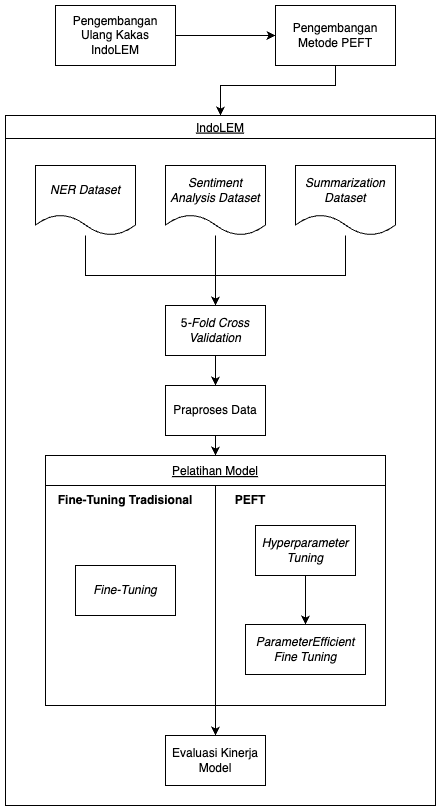
\includegraphics[height=0.6\textheight]{chapter-3/rancangan_solusi.png}
    \caption{Rancangan Solusi}
    \label{fig:rancangan-solusi}
\end{figure}

Sebelum bisa dilakukan pelatihan dan evaluasi model, kakas IndoLEM perlu dilakukan pengembangan ulang serta perlu dikembangkan metode PEFT pada kakas IndoLEM. Pengembangan ulang ini dilakukan agar pengembangan metode PEFT bisa dilakukan. Pengembangan ulang kakas IndoLEM  menggunakan beberapa pustaka, salah satunya adalah Transformers dan Torch. Pustaka Transformers diperlukan untuk melakukan pemuatan model, praproses data, dan penggunaan Trainer untuk standardisasi. Lalu, pustaka Torch digunakan untuk menggunakan CUDA yang memanfaatkan GPU untuk melatih model. Selain itu, pustaka Wandb dan Huggingface juga  dipakai untuk melakukan sinkronisasi pada \textit{cloud}. Dengan sinkronisasi ini, hasil pelatihan model dan hasil evaluasi dapat dilihat pada situsnya yang  memudahkan proses eksperimen. 

Pengembangan metode PEFT pada kakas IndoLEM  menggunakan pustaka Adapters. Model yang dimuat oleh pustaka Transformers perlu diinisiasi oleh pustaka Adapters untuk dapat berjalan menggunakan metode PEFT. Untuk dapat menjalankan proses pelatihan dengan metode PEFT, perlu menggunakan Trainer yang berasal dari pustaka Adapters yaitu AdapterTrainer yang  melakukan \textit{freeze} pada parameter model dan  menggunakan parameter yang sesuai dengan metode PEFT-nya tersebut.

Sesuai dengan banyaknya tugas evaluasi yang diimplementasikan, jumlah dari \textit{dataset} juga sebanyak tugas evaluasi tersebut, yaitu \nlptask. Setiap \textit{dataset}  dilakukan 5-\textit{fold cross validation} yang membagi setiap dataset menjadi 5 bagian \textit{dataset} validasi yang berbeda. Metode \textit{cross validation} ini sudah dilakukan pada kakas IndoLEM, sehingga \textit{dataset} sudah terbagi menjadi 5-\textit{fold}. Untuk setiap \textit{fold}-nya, \textit{dataset}  dilakukan praproses data, pelatihan model, dan evaluasi kinerja. Praproses data ini dilakukan dengan melakukan \textit{padding}, tokenisasi, dan juga mengatur \textit{mapping} dengan labelnya. 

Untuk proses pelatihan model  dibagi menjadi dua, yaitu dengan menggunakan \textit{fine-tuning} dan menggunakan metode PEFT. Pelatihan model  dilakukan pada lingkungan pelatihan yang sesuai yaitu pada lingkungkan \textit{cloud} yang menggunakan GPU khusus untuk pelatihan model. Pelatihan dengan \textit{fine-tuning} mengikuti \textit{hyperparameter} pada penelitian terkaitnya. Sedangkan, untuk metode PEFT  dilakukan \textit{hyperparameter tuning} untuk metode PEFT-nya.

Selanjutnya, untuk setiap hasil pelatihan model  dilakukan evaluasi pada dengan menggunakan \textit{dataset} validasi-nya. Metriks evaluasi yang digunakan tergantung pada tugas evaluasinya. Tugas evaluasi \textit{classification} yaitu NER dan \textit{sentiment analyisis}  menggunakan \textit{accuracy} dan F1 \textit{score}. Sedangkan, tugas evaluasi \textit{generation} yaitu \textit{summarization}  menggunakan ROUGE \textit{score}.



\chapter{Implementasi, Eksperimen, dan Hasil Evaluasi Eksperimen}
Bab ini menjelaskan proses implementasi dari rancangan solusi yang telah dikaji pada Bab \ref{sec:chapter-3} dalam menyelesaikan permasalahan utama tugas akhir, yaitu pemanfaatan berbagai metode PEFT pada kakas evaluasi IndoLEM. Selain itu, dijelaskan juga lingkungan, implementasi, dan eksperimen.

Berdasarkan rancangan solusi yang diajukan pada subbab \ref{sec:rancangan-solusi}, pembangunan ulang kakas IndoLEM diperlukan untuk mengimplementasi setiap metode PEFT. Model yang dipilih yaitu IndoBERT untuk tugas evaluasi \textit{classification} dan IndoT5 untuk tugas evaluasi \textit{generation} dilatih pada lingkungan eksperimen. Model yang telah dilatih dengan metode \textit{fine-tuning} tradisional dan metode PEFT dievaluasi untuk membandingkan kinerja dari setiap metode pada setiap tugas evaluasinya.

\section{Lingkungan}
\section{Pengembangan Ulang Kakas IndoLEM}
\label{sec:pengembangan-kakas}

Pengembangan ulang kakas IndoLEM ini diperlukan untuk memperbarui dan memperbaiki infrastruktur dari kakas tersebut. Pengembangan ini dilakukan pada lingkungan lokal pribadi, untuk keperluan eksperimen dilakukan pada lingkungan \textit{cloud} seperti yang sudah disebutkan pada subbab \ref{sec:lingkungan-eksperimen}.

\subsection{Persiapan Lingkungan Pengembangan}

Implementasi diawali dengan menyiapkan lingkungan pengembangan, untuk menyiapkan lingkungan pengembangan dilakukan dengan melakukan instalasi terhadap perangkat lunak dan pustaka yang dibutuhkan. Berikut merupakan \textit{requirements.txt} yang berisi pustaka yang perlu dilakukan intalasi yang bisa dilihat pada tabel \ref{table:requirements}

\begin{table}[h]
    \caption{Tabel \textit{requirements.txt}}
    \label{table:requirements}
    \begin{lstlisting}[language=bash]
    accelerate
    adapters==0.2.2
    datasets
    evaluate
    huggingface-hub
    numpy
    pandas
    scikit-learn
    seqeval
    torch
    transformers==4.40.*
    wandb
    nltk
    rouge_score
    indobenchmark-toolkit
    \end{lstlisting}
\end{table}

Untuk memudahkan pengembangan perlu membuat \textit{virtual environment} untuk mengenkapsulasi pustaka yang dipakai. \textit{Virtual environment} bisa dibuat dengan menggunakan Conda atau pustaka virtualenv. Untuk tugas akhir ini, digunakan Conda. \textit{Command} yang digunakan dapat dilihat pada tabel \ref{table:command-virtualenv}.

\begin{table}[h]
    \caption{Tabel \textit{command virtual environment}}
    \label{table:command-virtualenv}
    \begin{lstlisting}[language=bash]
    # Membuat virtual environment
    conda create env -n indolem python=3.11
    # Menjalankan virtual environment
    conda activate indolem
    # Melakukan instalasi pustaka 
    pip install -r requirements.txt
    \end{lstlisting}
\end{table}

\textit{Command} tersebut akan membuat \textit{virtual environment}, mengakitfkannya, dan melakukan instalasi pada versi Python dan pustaka yang dibutuhkan.

\subsection{Penguraian Argumen}
\label{sec:parse-arg}

Penguraian argumen dilakukan dengan menggunakan modul HfArgumentParser dari pustaka Transformers. Modul ini digunakan untuk memudahkan penguraian argumen karena argumen yang dipakai untuk model, pelatihan, dan evaluasi sudah diimplementasikan dari modul tersebut. Untuk argumen tambahan yang spesifik pada suatu tugas evaluasi perlu ditambahkan secara manual, sebagai contoh pada tugas evaluasi NER terdapat argumen \textit{return\_entity\_level\_metrics} yaitu menggunakan metriks evaluasi untuk level entitasnya.

\begin{table}[h]
    \caption{Tabel kode HfArgumentParser}
    \label{table:hfargumentparser}
    \begin{lstlisting}[language=python]
    parser = HfArgumentParser(
        [
            ModelArguments,
            DataTrainingArguments,
            TrainingArguments,
            AdapterArguments,
            WandbArguments,
        ]
    )

    if len(sys.argv) == 2 and sys.argv[1].endswith(".json"):
        # If we pass only one argument to the script and it's the path to a json file,
        # let's parse it to get our arguments.
        model_args, data_args, training_args, adapter_args, wandb_args = (
            parser.parse_json_file(json_file=os.path.abspath(sys.argv[1]))
        )
    else:
        model_args, data_args, training_args, adapter_args, wandb_args = (
            parser.parse_args_into_dataclasses()
        )
    \end{lstlisting}
\end{table}

Berdasarkan tabel \ref{table:hfargumentparser} terdapat 5 jenis argumen, yaitu model, \textit{data training}, pelatihan, \textit{adapter}, dan wandb. Argumen model digunakan untuk pemuatan model. Argumen \textit{data training} digunakan untuk pemuatan \textit{file} (latih, evaluasi, dan uji), \textit{padding}, maksimum sampel, maksimum sekuens, dan lain sebagainya yang berhubungan dengan \textit{dataset}. Lalu, argumen pelatihan merupakan \textit{hyperparemeter} yang digunakan pada proses pelatihan seperti \textit{learning rate, epoch, batch size}, dan lain sebagainya. Selanjutnya, argumen \textit{adapter} berfungsi sebagai konfigurasi untuk jenis metode PEFT beserta \textit{hyperparameter} yang digunakannya. Terakhir, merupakan argumen wandb yang digunakan untuk konfigurasi sinkronisasi pada hasil evaluasi ke \textit{cloud}.

\subsection{Praproses \textit{Dataset}}
\label{sec:praproses}

Praproses \textit{dataset} diperlukan agar model dapat memproses \textit{dataset} dengan konteks yang sesuai. Konteks yang dimaksud adalah, model dapat memahami \textit{metadata} dari \textit{dataset}, sehingga mampu mengetahui setiap bagian data yang merupakan bagian dari teks atau label. Praproses \textit{dataset} ini berbeda untuk setiap tugas evaluasi karena karakteristik dari tugas evaluasinya yang berbeda juga.

\subsubsection{Praproses Data NER}

Tugas evaluasi NER merupakan jenis tugas \textit{classification} pada level token yang berarti setiap token akan diklasifikasikan dengan label tertentu. Pada kakas IndoLEM, untuk tugas evaluasi NER terdapat dua jenis \textit{dataset}, yaitu NERUI dan NERUGM. Kedua \textit{dataset} tersebut mempunyai label yang berbeda berikut merupakan label pada setiap \textit{dataset}-nya dapat dilihat pada tabel \ref{table:label-ner}.

\begin{table}[h]
    \vspace{0.25cm}
    \caption{Tabel label \textit{dataset} NER}
    \label{table:label-ner}
    \begin{center}
        \begin{tabular}{|l|l|}
            \hline \rowcolor{black!10}
            \multicolumn{1}{|c|}{\textbf{NERUI}} & \multicolumn{1}{|c|}{\textbf{NERUI}} \\ \hline
            B-LOCATION & B-LOCATION \\ \hline
            B-ORGANIZATION & B-ORGANIZATION \\ \hline
            B-PERSON & B-PERSON \\ \hline
            - & B-QUANTITY \\ \hline
            - & B-TIME \\ \hline
            I-LOCATION & I-LOCATION \\ \hline
            I-ORGANIZATION & I-ORGANIZATION \\ \hline
            I-PERSON & I-PERSON \\ \hline
            - & I-QUANTITY \\ \hline
            - & I-TIME \\ \hline
            O & O \\ \hline
        \end{tabular}
    \end{center}
\end{table}

Label tersebut diperlukan untuk melakukan \textit{mapping} antara id dengan labelnya yang akan digunakan pada konfigurasi model. \textit{Padding} juga dilakukan berdasarkan panjang sekuens maksimum yang didefinisikan melaluai argumen \textit{data training}. Selanjutnya, tokenisasi akan dilakukan terhadap \textit{dataset} tersebut. Implementasi dari fungsi tokenisasi tersebut dapat dilihat pada tabel \ref{table:tokenisasi-ner}.

\begin{table}[h]
    \caption{Tabel fungsi tokenisasi NER}
    \label{table:tokenisasi-ner}
    \begin{lstlisting}[language=python]
    def tokenize_and_align_labels(examples):
        tokenized_inputs = tokenizer(
            examples[text_column_name],
            padding=padding,
            truncation=True,
            max_length=data_args.max_seq_length,
            is_split_into_words=True,
        )
        labels = []

        for i, label in enumerate(examples[label_column_name]):
            word_ids = tokenized_inputs.word_ids(batch_index=i)
            previous_word_idx = None
            label_ids = []
            for word_idx in word_ids:
                if word_idx is None:
                    label_ids.append(-100)
                elif word_idx != previous_word_idx:
                    label_ids.append(label_to_id[label[word_idx]])
                else:
                    if data_args.label_all_tokens:
                        label_ids.append(b_to_i_label[label_to_id[label[word_idx]]])
                    else:
                        label_ids.append(-100)
                previous_word_idx = word_idx

            labels.append(label_ids)
        tokenized_inputs["labels"] = labels
        return tokenized_inputs
    \end{lstlisting}
\end{table}

Tokenisasi dilakukan dengan menggunakan modul Tokenizer pada pustaka Transformers. Fungsi tokenisasi pada tabel \ref{table:tokenisasi-ner} mengabaikan token spesial [CLS] dan [SEP] yang muncul dari hasil tokenisasi model berbasi BERT. Token spesial tersebut diubah menjadi -100 agar bisa diabaikan dari perhitungan metriks evaluasinya. Sehingga, hanya token yang berkorespondensi terhadap sebuah label saja yang dapat dievaluasi.

\subsubsection{Praproses Data \textit{Sentiment Analysis}}

Tugas evaluasi \textit{sentiment analysis} merupakan jenis tugas \textit{classification} sama seperti NER, hanya perbedaannya pada level klasifikasi yang digunakan. Jika pada NER klasifikasi dilakukan pada level token, pada \textit{sentiment analysis} klasifikasi dilakukan pada level teks yang merupakan gabungan dari beberapa token. \textit{Dataset} dari \textit{sentiment analysis} berupa \textit{file} CSV yang berisi dari dua kolom yaitu \textit{sentence} dan \textit{labels}. Kolom \textit{sentence} merupakan teks yang mengandung sentiment tertentu. Sementara kolom \textit{labels} menandakan sentimen dari teks tersebut, dengan nilai 0 berupa sentimen negatif dan  nilai 1 berupa sentiment positif.

\begin{table}[h]
    \caption{Tabel fungsi tokenisasi \textit{sentiment analysis}}
    \label{table:tokenisasi-sentiment}
    \begin{lstlisting}[language=python]
        def preprocess_function(examples):
            # Tokenize the texts
            args = (
                (examples[sentence1_key],)
                if sentence2_key is None
                else (examples[sentence1_key], examples[sentence2_key])
            )
            result = tokenizer(
                *args, padding=padding, max_length=max_seq_length, truncation=True
            )

            # Map labels to IDs
            if label_to_id is not None and "labels" in examples:
                result["labels"] = [
                    (label_to_id[l] if l != -1 else -1) for l in examples["labels"]
                ]
            return result
    \end{lstlisting}
\end{table}

Pada tugas evaluasi \textit{sentiment analysis} juga diperlukan \textit{mapping} antara label dengan idnya, sehingga model mampu mengetahui label yang dilatih. Fungsi tokenisasi \textit{sentiment analysis} yang dapat dilihat pada tabel \ref{table:tokenisasi-sentiment} menggunakan modul Tokenizer dari pustaka Transformers. Fungsi tersebut terdapat \textit{sentence1\_key} dan juga \textit{sentence2\_key}, yang berguna apabila terdapat dua kolom teks pada \textit{dataset}, tetapi pada IndoLEM \textit{dataset sentiment analysis} hanya mempunyai satu kolom teks. Sehingga, \textit{sentence2\_key} tidak digunakan. 

\subsubsection{Praproses Data \textit{Summarization}}

Tugas evaluasi \textit{summarization} merupakan jenis tugas \textit{generation} yang berbeda dengan jenis tugas \textit{classification}. Tugas \textit{generation} memerlukan generasi teks untuk dapat dilakukan evaluasi, pada konteks ini yaitu membuat ringkasan dari teks. \textit{Dataset} yang digunakan pada IndoLEM untuk tugas evaluasi \textit{summarization} adalah \textit{dataset} IndoSUM. \textit{Dataset} ini berisi \textit{file} dengan format JSONL dengan masing-masing objek dapat dilihat pada tabel \ref{table:data-summarization}.

\begin{table}[h]
    \vspace{0.25cm}
    \caption{Tabel data \textit{summarization}}
    \label{table:data-summarization}
    \begin{center}
        \begin{tabular}{|l|l|}
            \hline \rowcolor{black!10}
            \multicolumn{1}{|c|}{\textbf{Objek}} & \multicolumn{1}{|c|}{\textbf{Deskripsi}} \\ \hline
            id & nilai unik untuk setiap artikel \\ \hline
            paragraphs & \textit{list} dari paragraf yang berasal dari artikel \\ \hline
            summary & ringkasan dari artikel, disimpan sebagai \textit{list} dari kalimat \\ \hline 
            gold\_labels & label ekstraktif dari setiap kalimat pada artikel \\ \hline
            category & kategori dari artikel \\ \hline
            source & sumber artikel \\ \hline
            source\_url & URL dari artikel \\ \hline
        \end{tabular}
    \end{center}
\end{table}

Dari data yang dapat dilihat pada tabel \ref{table:data-summarization}, terdapat 7 objek  pada \textit{dataset}. Namun, pada tugas evaluasi ini hanya akan digunakan dua objek yaitu \textit{paragraphs} dan \textit{summary} karena tugas \textit{summarization} membutuhkan teks asli sebelum diringkas dan hasil ringkasannya. Objek yang lain selain dua yang digunakan bisa diabaikan saja. \textit{Dataset} ini perlu dipraproses terlebih dahulu menggunakan fungsi yang dapat dilihat pada tabel \ref{table:tokensisasi-summ}.

\begin{table}[h]
    \caption{Tabel fungsi tokenisasi \textit{summarization}}
    \label{table:tokensisasi-summ}
    \begin{lstlisting}[language=python]
    def preprocess_function(examples):
        if is_indosum:
            examples[text_column] = paragraph_to_text(examples[text_column])
            examples[summary_column] = summary_to_text(examples[summary_column])

        inputs = [prefix + inp for inp in inputs]
        model_inputs = tokenizer(
            inputs,
            max_length=data_args.max_source_length,
            padding=padding,
            truncation=True,
        )

        labels = tokenizer(
            text_target=targets,
            max_length=max_target_length,
            padding=padding,
            truncation=True,
        )

        if padding == "max_length" and data_args.ignore_pad_token_for_loss:
            labels["input_ids"] = [
                [(l if l != tokenizer.pad_token_id else -100) for l in label]
                for label in labels["input_ids"]
            ]

        model_inputs["labels"] = labels["input_ids"]
        return model_inputs
    \end{lstlisting}
\end{table}

Berdasarkan tabel \ref{table:tokensisasi-summ}, tokenisasi dilakukan dengan mengolah objek \textit{paragraphs} menjadi \textit{list} dari teks. Setiap paragraf terdiri dari beberapa kalimat, dan setiap kalimat terdiri dari beberapa teks. Untuk \textit{text\_column} yang merupakan objek \textit{paragraphs} akan diolah menjadi \textit{list} dari teks. Hal yang sama berlaku juga untuk \textit{summary\_column}, hanya saja objek ini merupakan \textit{summary} yang berisi kalimat. Selain itu, tugas evaluasi \textit{summarization} ini terdapat \textit{prefix} yang berguna pada beberapa model tertentu. Tokenisasi juga menggunakan modul \textit{tokenizer} dari pustaka Transformers.

\subsection{Pemuatan Konfigurasi Model}

Untuk dapat melakukan pelatihan dan evaluasi terhadap model, terlebih dahulu model perlu dimuat. Pemuatan model ini menggunakan konfigurasi yang dimuat dari penguraian argumen pada subbab \ref{sec:parse-arg}. Argumen model akan dimuat ke dalam model sehingga model bisa dipakai. Model akan dimuat dengan menggunakan modul yang relevan dari pustaka Transformers.

\begin{table}[h]
    \caption{Tabel kode pemuatan model \textit{summarization}}
    \label{table:kode-model-summ}
    \begin{lstlisting}[language=python]
    model = AutoModelForSeq2SeqLM.from_pretrained(
        model_args.model_name_or_path,
        from_tf=bool(".ckpt" in model_args.model_name_or_path),
        config=config,
        cache_dir=model_args.cache_dir,
        revision=model_args.model_revision,
        token=True if model_args.token else None,
    )
    \end{lstlisting}
\end{table}

Pada tabel \ref{table:kode-model-summ} dimuat model AutoModelForSeq2SeqLM yang merupakan model \textit{sequence to sequence} yang merupakan model \textit{encoder decoder}. Modul AutoModel ini akan menghasilkan model berdasarkan dari konfigurasi \textit{model\_args} yang dimasukkan pada modul tersebut. Untuk tugas evaluasi \textit{summarization} yang menggunakan model IndoT5 akan menghasilkan model tersebut juga. Berbeda untuk tugas \textit{classification}, cukup dengan menyatakan AutoModel saja sudah cukup untuk menghasilkan model yang sesuai. Pada konteks ini, model yang digunakan untuk NER dan \textit{sentiment analysis} adalah IndoBERT yang berbasis BERT.

\subsection{Perhitungan Metriks Evaluasi}
\label{sec:metriks-evaluasi}

Metriks evaluasi yang digunakan pada setiap tugas evaluasi tidak sama semuanya. Metriks yang digunakan untuk tugas \textit{classification} adalah \textit{accuracy} dan F1 \textit{score}. Sedangkan, pada tugas \textit{generation} adalah ROUGE \textit{score}. Perhitungan metriks evaluasi ini dilakukan saat proses evaluasi dengan menggunakan fungsi \textit{compute\_metrics}.

\begin{table}[h]
    \caption{Tabel fungsi \textit{compute\_metrics}}
    \label{table:compute-metrics}
    \begin{lstlisting}[language=python]
    def compute_metrics(p):
        logits, labels = p
        predictions = np.argmax(logits, axis=1)

        return {
            "accuracy": accuracy_score(labels, predictions),
            "precision": precision_score(labels, predictions, average="macro"),
            "recall": recall_score(labels, predictions, average="macro"),
            "f1": f1_score(labels, predictions, average="macro"),
        }
    \end{lstlisting}
\end{table}

Pada tabel \ref{table:compute-metrics}, fungsi perhitungan metriks evaluasinya merupakan fungsi yang dipakai untuk tugas \textit{classification}. Fungsi tersebut memanfaatkan modul seqeval untuk melakukan perhitungan setiap metriksnya. Terdapat perbeedaan pada fungsi yang dipakai pada tugas \textit{classifcation}, NER menggunakan \textit{entity\_level\_metrics} yang berarti perhitungan evaluasinya berdasarkan pada entitasnya yang berbeda dengan \textit{sentiment analysis}. Untuk tugas \textit{generation} yaitu \textit{summarization} menggunakan ROUGE \textit{score}.

\subsection{Pemuatan Trainer untuk Pelatihan dan Evaluasi Model}

Untuk pelatihan dan evaluasi model dibutuhkan standardisasi agar kode yang digunakan pada setiap tugas tidak berbeda. Modul Trainer dari pustaka Transformers digunakan untuk pelatihan dan evaluasi model. Setiap komponen yang sudah disebutkan sebelumnya akan dimuat pada modul Trainer. Setiap tugas evaluasi akan menggunakan implementasi yang sama yang bisa dilihat pada tabel \ref{table:kode-trainer}.

\begin{table}[h]
    \caption{Tabel kode implementasi Trainer}
    \label{table:kode-trainer}
    \begin{lstlisting}[language=python]
    trainer = Trainer(
        model=model,
        args=training_args,
        train_dataset=train_dataset if training_args.do_train else None,
        eval_dataset=eval_dataset if training_args.do_eval else None,
        tokenizer=tokenizer,
        data_collator=data_collator,
        compute_metrics=compute_metrics,
    )

    trainer.train(resume_from_checkpoint=checkpoint)
    trainer.evaluate()
    \end{lstlisting}
\end{table}

Kode implementasi Trainer pada tabel \ref{table:kode-trainer} memuat modul Trainer dan memanggil metode \textit{train} dan \textit{evaluate} untuk melakukan pelatihan dan evaluasi. Modul Trainer membutuhkan beberapa argumen yang dimuat. Argumen tersebut dimuat dari komponen-komponen yang sudah disebutkan pada subbab sebelumnya. Argumen untuk pelatihan, dan model didapat dari hasil penguraian argumen pada \ref{sec:parse-arg}. Untuk \textit{tokenizer} dan \textit{dataset} pelatihan dan evaluasi dimuat dari hasil praproses data pada \ref{sec:praproses}. Lalu, untuk \textit{compute\_metrics} fungsinya dimuat dari metriks evaluasi pada \ref{sec:metriks-evaluasi}. 

\section{Pengembangan Metode PEFT pada Kakas IndoLEM}

Pengembangan metode PEFT pada kakas IndoLEM menggunakan pustaka Adapters. Pustaka tersebut tidak hanya mengimplementasikan setiap metode saja, tetapi terdapat fungsionalitas untuk menggabungkan beberapa metode PEFT. Pada subbab sebelumnya yaitu subbab \ref{sec:pengembangan-kakas}, kakas IndoLEM dikembangkan ulang agar mampu untuk mengimplementasikan metode PEFT. Implementasi tersebut  mengubah beberapa komponen, yaitu komponen model dan trainer. Metode PEFT  melakukan \textit{freeze} pada parameter model sehingga pada proses pelatihan tidak  mengubah parameter model melainkan parameter dari metode PEFT tersebut.

\begin{table}[h]
    \caption{Tabel kode pemuatan model Adapters}
    \label{table:kode-model-adapters}
    \begin{lstlisting}[language=python]
    model = AutoAdapterModel.from_pretrained(
        model_args.model_name_or_path,
        from_tf=bool(".ckpt" in model_args.model_name_or_path),
        config=config,
        cache_dir=model_args.cache_dir,
        revision=model_args.model_revision,
        token=True if model_args.token else None,
        ignore_mismatched_sizes=model_args.ignore_mismatched_sizes,
    )
    \end{lstlisting}
\end{table}

Pada kode pemuatan model Adapters yang bisa dilihat pada tabel \ref{table:kode-model-adapters}, model dimuat dengan modul AutoAdapterModel dari pustaka Adapters. Hal ini dilakukan untuk \textit{support} metode PEFT yang lebih baik berdasarkan dari dokumentasi dari pustakanya. Berbeda dari tabel \ref{table:kode-model-summ} yang menggunakan AutoModel dari pustaka Transformers, AutoAdapterModel memberikan fungsionalitas yang lebih baik untuk metode PEFT, salah satunya adalah untuk membandingkan parameter yang  dilatih dibanding dengan parameter asli dari modelnya.

\begin{table}[h]
    \caption{Tabel kode implementasi AdapterTrainer}
    \label{table:kode-adaptertrainer}
    \begin{lstlisting}[language=python]
    setup_adapter_training(model, adapter_args)
    trainer = AdapterTrainer(
        model=model,
        args=training_args,
        train_dataset=train_dataset if training_args.do_train else None,
        eval_dataset=eval_dataset if training_args.do_eval else None,
        tokenizer=tokenizer,
        data_collator=data_collator,
        compute_metrics=compute_metrics,
    )

    trainer.train(resume_from_checkpoint=checkpoint)
    trainer.evaluate()
    \end{lstlisting}
\end{table}

Selanjutnya, untuk proses pelatihan perlu disiapkan untuk menggunakan metode PEFT. Implementasinya menggunakan modul AdapterTrainer dari pustaka Adapters juga. Model perlu disiapkan untuk pelatihan dengan metode PEFT dengan menggunakan fungsi \textit{setup\_adapter\_training}. Fungsi tersebut  melakukan \textit{freeze} pada parameter model dan hanya  mengubah parameter dari metode PEFT yang digunakan. Argumen untuk \textit{adapter} dimuat dari hasil pengurain argumen pada \ref{sec:parse-arg}, argumen tersebut berisi jenis metode PEFT serta \textit{hyperparameter} yang digunakan pada proses pelatihan. Proses pelatihan metode PEFT berbeda dengan pelatihan dengan metode \textit{fine-tuning} tergantung dari karakteristik dari metode tersebut. Pustaka Adapters mengimplementasikannya dengan menambahkan semacam \textit{adapter} pada model, sehingga \textit{adapter} tersebut yang dilatih bukan modelnya. Parameter dari \textit{adapter} tersebut relatif lebih kecil daripada parameter model.

\section{Pelatihan Model}

Pelatihan model dilakukan pada lingkungan eksperimen yang telah disebutkan pada subbab \ref{sec:lingkungan-eksperimen}. Pelatihan dilakukan dengan \textit{bash script} yang  dijalankan pada \textit{shell} untuk memudahkan reka ulang dari eksperimen tersebut. Untuk setiap tugas evaluasi terdapat \textit{bash script} yang  menjalankan semua eksperimen, yaitu \textit{fine-tuning}, \methodPEFT.

\begin{figure}[h]
    \centering
    \caption{Struktur \textit{file} eksperimen}
    \label{fig:file-eksperimen}
    \begin{forest}
        for tree={
            font=\ttfamily,
            grow'=0,
            child anchor=west,
            parent anchor=south,
            anchor=west,
            calign=first,
            edge path={
                \noexpand\path [draw, \forestoption{edge}]
                (!u.south west) +(7.5pt,0) |- node[fill,inner sep=1.25pt] {} (.child anchor)\forestoption{edge label};
            },
            before typesetting nodes={
                if n=1
                    {insert before={[,phantom]}}
                    {}
            },
            fit=band,
            before computing xy={l=15pt},
        }
    [run\_sentiment.sh
        [script
            [run\_sentiment\_base.sh]
            [run\_sentiment\_lora.sh]
            [run\_sentiment\_pt.sh]
            [run\_sentiment\_seq\_bn.sh]
            [run\_sentiment\_unipelt.sh]
        ]
    ]
    \end{forest}
\end{figure}

Pada gambar \ref{fig:file-eksperimen}, dengan melakukan pemanggilan pada {\ttfamily run\_sentiment.sh}  menjalankan semua eksperimen yang ada pada folder {\ttfamily script}. Setiap \textit{script}  menjalankan eksperimen sesuai dari konfigurasi yang telah ditentukan pada \textit{script} tersebut. Konfigurasi yang ditentukan tersebut  diterima sebagai argumen pada kakas IndoLEM. Untuk setiap \textit{hyperparameter} yang digunakan untuk pelatihan dapat dilihat pada tabel \ref{table:hyperparameter-train}.

\begin{table}[h]
    \centering
    \caption{Tabel \textit{hyperparameter} pelatihan}
    \label{table:hyperparameter-train}
    \begin{tabular}{|c|l|c|}
        \hline \rowcolor{black!10}
        \textbf{Tugas} & \multicolumn{1}{|c|}{\textbf{Argumen}} & \textbf{Nilai} \\ \hline
        \multirow{9}{*}{\textit{NER}} & model & "indolem/indobert-base-uncased" \\ \cline{2-3}
                                      & train batch size & 16 \\ \cline{2-3}
                                      & eval batch size & 64 \\ \cline{2-3}
                                      & epochs & 100 \\ \cline{2-3}
                                      & learning rate & 5e-5 \\ \cline{2-3}
                                      & max sequence length & 128 \\ \cline{2-3}
                                      & text column names & "tokens" \\ \cline{2-3}
                                      & label column names & "ner\_tags" \\ \cline{2-3}
                                      & return entity level metrics & true \\ \cline{2-3}
                                      & seed & 42 \\ \hline
        \multirow{7}{*}{\textit{sentiment analysis}} & model & "indolem/indobert-base-uncased" \\ \cline{2-3}
                                                     & batch size & 30 \\ \cline{2-3}
                                                     & epochs & 20 \\ \cline{2-3}
                                                     & learning rate & 5e-5 \\ \cline{2-3}
                                                     & max sequence length & 200 \\ \cline{2-3}
                                                     & seed & 42 \\ \cline{2-3}
                                                     & label names & "labels" \\ \hline
        \multirow{14}{*}{\textit{summarization}} & model & "LazarusNLP/IndoNanoT5-base" \\ \cline{2-3}
                                                & train batch size & 4 \\ \cline{2-3}
                                                & eval batch size & 8 \\ \cline{2-3}
                                                & epochs & 5 \\ \cline{2-3}
                                                & learning rate & 1e-5 \\ \cline{2-3}
                                                & max source length & 512 \\ \cline{2-3}
                                                & max target length & 512 \\ \cline{2-3}
                                                & num beams & 5 \\ \cline{2-3}
                                                & weight decay & 0.01 \\ \cline{2-3}
                                                & patience & 5 \\ \cline{2-3}
                                                & seed & 42 \\ \cline{2-3}
                                                & text column & paragraphs \\ \cline{2-3}
                                                & summary column & summary \\ \cline{2-3}
                                                & source prefix & "summarize: " \\ \cline{2-3}
                                                & pad to max length & true \\ \cline{2-3}
                                                & predict with generate & true \\ \cline{2-3}
                                                & bf16 & true \\ \hline
    \end{tabular}
\end{table}

Untuk pelatihan model NER terdapat dua \textit{dataset} yang  digunakan yaitu NERUGM dan NERUI. Sedangkan, untuk tugas \textit{sentiment analysis} dan \textit{summarization} menggunakan satu dataset. Selain itu, untuk tugas NER terdapat argumen "return entity level metrics" dengan nilai "true" yang berarti penilaian metriks evaluasinya  dinilai pada level entitas. Ini mengikuti eksperimen yang sebelumnya sudah dilakukan pada IndoLEM.

Terdapat perbedaan pada \textit{hyperparameter} yang digunakan untuk tugas \textit{summarization} karena argumen yang digunakan mengikuti eksperimen pada IndoT5 bukan pada IndoLEM. Terdapat juga argumen "predict with generate" dengan nilai "true" karena tugas \textit{summarization} perlu menghasilkan hasil ringkasan untuk dapat dievaluasi. Selain itu, nilai argumen "bf16" bernilai "true" karena presisi "bf16" dianggap bisa mempercepat proses pelatihan untuk model T5 yang digunakan. Pada tugas ini perlu menambahkan argumen "source prefix" yang bernilai "summarize: " khusus unutk penggunaan model T5 pada tugas \textit{summarization}.

\begin{table}[h]
    \centering
    \caption{Tabel \textit{hyperparameter} metode PEFT}
    \label{table:hyperparameter-PEFT}
    \begin{tabular}{|l|l|c|}
        \hline \rowcolor{black!10}
        \multicolumn{1}{|c|}{\textbf{Metode}} & \multicolumn{1}{|c|}{\textbf{Argumen}} & \textbf{Nilai} \\ \hline
        LoRA & ranks & [8, 16] \\ \hline
        Prefix Tuning & prefix length & [10, 20, 30] \\ \hline
        Bottleneck Adapter & \multicolumn{1}{|c|}{-} & - \\ \hline
        UniPELT & \multicolumn{1}{|c|}{-}  & - \\ \hline
    \end{tabular}
\end{table}

Pada pelatihan dengan metode PEFT  menggunakan \textit{hyperparameter} pelatihan seperti pada tabel \ref{table:hyperparameter-train}. Untuk setiap metode PEFT terdapat \textit{hyperparameter} yang sesuai dengan metode PEFT tersebut. Perlu dilakukan \textit{hyperparameter tuning} untuk \textit{hyperparameter} metode PEFT. Seperti yang bisa dilihat pada tabel \ref{table:hyperparameter-PEFT}, untuk metode LoRA dilakukan eksperimen dengan argumen "ranks" dengan nilai 8 dan 16. Lalu, untuk metode Prefix Tuning dilakukan eksperimen dengan argumen "prefix tuning" dengan nilai 10, 20, dan 30. Selain itu, yaitu metode Bottleneck Adapter dan UniPELT tidak menggunakan argumen tambahan, hal ini dilakukan karena metode tersebut memang spesifik diimplementasikan pada pustaka Adapters sesuai dengan penelitian terkaitnya.

\section{Evaluasi Model}


\chapter{Penutup}

Bab Kesimpulan dan Saran akan menjadi bagian akhir dan penutup dari penelitian tugas akhir ini. Bab ini akan membahas kesimpulan yang berisi ketercapaian tujuan penelitian tugas akhir dengan permasalahan yang diselesaikan dalam penelitian tugas akhir. Selain itu, bab ini akan membahas saran yang dapat dilakukan untuk pengembangan atau penelitian selanjutnya.

\section{Kesimpulan}

\section{Saran}

%---------------------------------------------------------------%

% Daftar pustaka
\printbibliography

% Setting judul lampiran
\titlespacing*{\chapter}{0pt}{0pt}{0pt}
\titlespacing*{\section}{0pt}{0pt}{*1}

% Setting judul anak lampiran
\titleformat*{\section}{\bfseries}

\appendix

\chapter{\textit{Hyperparameter} pelatihan}

\begin{table}[h]
    \centering
    \caption{\textit{Hyperparameter} pelatihan}
    \label{appendix:hyperparameter-train}
    \resizebox{\textwidth}{!}{
        \begin{tabular}{|c|l|c|}
            \hline 
            \textbf{Tugas} & \multicolumn{1}{|c|}{\textbf{Argumen}} & \textbf{Nilai} \\ \hline
            \multirow{9}{*}{\textit{NER}} & \texttt{model} & "indolem/indobert-base-uncased" \\ \cline{2-3}
                                          & \texttt{train\_batch\_size} & 16 \\ \cline{2-3}
                                          & \texttt{eval\_batch\_size} & 64 \\ \cline{2-3}
                                          & \texttt{epochs} & 100 \\ \cline{2-3}
                                          & \texttt{learning\_rate} & 5e-5 \\ \cline{2-3}
                                          & \texttt{max\_sequence\_length} & 128 \\ \cline{2-3}
                                          & \texttt{text\_column\_names} & "tokens" \\ \cline{2-3}
                                          & \texttt{label\_column\_names} & "ner\_tags" \\ \cline{2-3}
                                          & \texttt{return\_entity\_level\_metrics} & true \\ \cline{2-3}
                                          & \texttt{seed} & 42 \\ \hline
            \multirow{7}{*}{\textit{Sentiment Analysis}} & \texttt{model} & "indolem/indobert-base-uncased" \\ \cline{2-3}
                                                         & \texttt{batch\_size} & 30 \\ \cline{2-3}
                                                         & \texttt{epochs} & 20 \\ \cline{2-3}
                                                         & \texttt{learning\_rate} & 5e-5 \\ \cline{2-3}
                                                         & \texttt{max\_sequence\_length} & 200 \\ \cline{2-3}
                                                         & \texttt{seed} & 42 \\ \cline{2-3}
                                                         & \texttt{label\_names} & "labels" \\ \hline
            \multirow{14}{*}{\textit{Summarization}} & \texttt{model} & "lazarusnlp/indonanot5-base" \\ \cline{2-3}
                                                    & \texttt{train\_batch\_size} & 4 \\ \cline{2-3}
                                                    & \texttt{eval\_batch\_size} & 8 \\ \cline{2-3}
                                                    & \texttt{epochs} & 5 \\ \cline{2-3}
                                                    & \texttt{learning\_rate} & 1e-5 \\ \cline{2-3}
                                                    & \texttt{max\_source\_length} & 512 \\ \cline{2-3}
                                                    & \texttt{max\_target\_length} & 512 \\ \cline{2-3}
                                                    & \texttt{num\_beams} & 5 \\ \cline{2-3}
                                                    & \texttt{weight\_decay} & 0.01 \\ \cline{2-3}
                                                    & \texttt{patience} & 5 \\ \cline{2-3}
                                                    & \texttt{seed} & 42 \\ \cline{2-3}
                                                    & \texttt{text\_column} & paragraphs \\ \cline{2-3}
                                                    & \texttt{summary\_column} & summary \\ \cline{2-3}
                                                    & \texttt{source\_prefix} & "summarize: " \\ \cline{2-3}
                                                    & \texttt{pad\_to\_max\_length} & true \\ \cline{2-3}
                                                    & \texttt{predict\_with\_generate} & true \\ \cline{2-3}
                                                    & \texttt{bf16} & true \\ \hline
        \end{tabular}
    }
\end{table}


\end{document}
